% Apresentação feita para o evento IC 40 ANOS
% Mestrado IC-UNICAMP
% Setembro 2009
% Author: Thiago Alvarenga Lechuga
% IC-UNICAMP
% http://www.ic.unicamp.br/~079699
%
\documentclass[red, cover=invisible, theme=Warsaw]{myslides}
\usepackage[brazil]{babel}
% \usepackage[utf8]{inputenc}

%adicionando numero de paginas
\usepackage{rodape}
\usepackage{pgfpages}

%poder criar tabelas com multirow
\usepackage{multirow}

%para adicionar codigo
\usepackage{listings}

%%%%%%%%%%%%%%%%%%%%%%%%%%%%%%%
%configurações para códigos inseridos
\lstset{
    language=XML,                   % choose the language of the code
    basicstyle=\footnotesize,       % the size of the fonts that are used for the code
    numbers=left,                   % where to put the line-numbers
    numberstyle=\footnotesize,      % the size of the fonts that are used for the line-numbers
    stepnumber=1,                   % the step between two line-numbers. If it's 1 each line will be numbered
    numbersep=10pt,                 % how far the line-numbers are from the code
    backgroundcolor=\color{white},  % choose the background color. You must add \usepackage{color}
    showspaces=false,               % show spaces adding particular underscores
    showstringspaces=false,         % underline spaces within strings
    showtabs=false,                 % show tabs within strings adding particular underscores
    frame=single,                   % adds a frame around the code
    tabsize=2,                      % sets default tabsize to 2 spaces
    captionpos=b,                   % sets the caption-position to bottom
    breaklines=true,                % sets automatic line breaking
    breakatwhitespace=false,        % sets if automatic breaks should only happen at whitespace
    escapeinside={\%*}{*)}         % if you want to add a comment within your code
%     extendedchars=\true,
%     inputencoding=utf8   
    }


%%%%%%%%%%%%%%%%%%%%%%%%%%%%%%%%

\setbeamertemplate{footline}[rodape]


\setbeameroption{hide notes}
%\setbeameroption{show notes}
%\setbeameroption{show notes on second screen=right}
%\setbeameroption{show only notes}

\begin{document}
%retirando o apendix da contagem d epaginas
%\renewcommand{\inserttotalframenumber}{14}

\title[Execução de Workflows WS-BPEL em CoCs]{Uma Infraestrutura Para a Execução de Workflows WS-BPEL em Clusters de Clusters}
\author{Thiago Alvarenga Lechuga}
\date{21/10/2010}
\logo{
\includegraphics[scale=0.1]{imagens/logoHD.jpg} }

\begin{frame}
\titlepage
Orientadora: Maria Beatriz Felgar de Toledo

Agência Financiadora: FAPESP
\end{frame}

\begin{frame}[plain]\frametitle{Sumário}
\small\tableofcontents
\end{frame}


%início da apresentação

\section{Introdução}
	
    \begin{frame}
	\begin{center}
	{\Huge Introdução}
	\end{center}
    \end{frame}
    
    \subsection*{Introdução}
    \begin{frame} \frametitle{Introdução}
	\begin{itemize}
	    \item Motivação para os \textit{Clusters} de \textit{Clusters}.
		\note[item]{\textbf{CoC:=}Continuam sendo uma solução para a demanda computacional. Compartilhar Clusters entre instituições}
	    \item Tarefas complexas precisam ser facilmente compostas e executadas, mantendo suas dependências.
	    \begin{itemize}
		    \item \textit{Workflow}?
			\note[item]{\textbf{WF:=}Automação de um processo de negócio, em parte ou como um todo, onde documentos, informações ou tarefas são transferidos de um participante para outro de acordo com um grupo de regras}
		    \item Padrões atuais para a composição de serviços em sistemas distribuídos heterogêneos ainda são inadequadas.
		    \item Requisitos específicos que devem ser considerados.
			\note[item]{\textbf{Requisitos:=}Seleção de recursos baseada em requisitos não-funcionais}
		    \item BPEL é um forte candidato (Serviços Web).
	    \end{itemize}	    
	\end{itemize}	
    \end{frame}
    
    \subsection{Objetivos}
	\begin{frame} \frametitle{Objetivos}
		\begin{itemize}
		    \item Extensão à linguagem WS-BPEL.
		    \item Especificação e seleção de recursos baseada em:
			\begin{itemize}
			 \item Requisitos de QoS;
			 \item Recursos computacionais requeridos para a execução de cada serviço.
			\end{itemize}
		    \item Proposta de arquitetura para a execução de \textit{workflows} em CoCs.
		    \item Implementação da arquitetura proposta em um ambiente de produção.
		    \item Especificação e implementação de um problema real no ambiente criado.
	    \end{itemize}		
	\end{frame}

\section{Fundamentos}
    \begin{frame}
	\begin{center}
	{\Huge Fundamentos}
	\end{center}
    \end{frame}     

    \subsection{SOA e Serviços Web}
	\begin{frame}\frametitle{SOA e Serviços Web}
	    \begin{itemize}
	     \item Emergiram como uma solução para a comunicação entre aplicações.
	     \item SOA faz uso extensivo da tecnologia de WS de maneira a definir uma estrutura distribuída, independente de plataforma e linguagem de programação.
	     \item Interoperabilidade.
	    \end{itemize}
	\end{frame}
	
	\begin{frame}\frametitle{Camadas Básicas}
	    \begin{itemize}
	     \item Descoberta: UDDI.
	     \item Descrição: WSDL.
	     \item Comunicação: SOAP.
	    \end{itemize}
	    \begin{center}
		\begin{figure}
		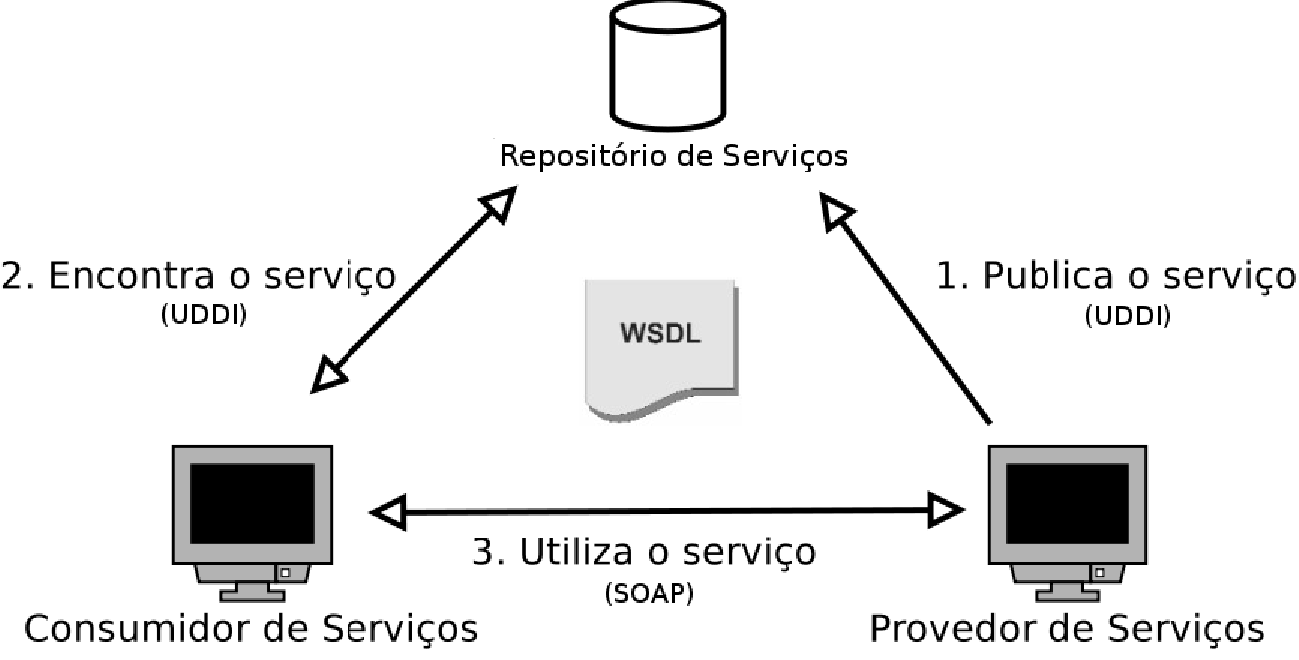
\includegraphics[scale=0.35]{imagens/SOA.pdf}
		\caption{Padrões SOA estabelecidos.}
		\end{figure}					
	    \end{center}
	\end{frame}
    
	\begin{frame}\frametitle{WS-Addressing}
	    \begin{itemize}
	    \item Especificação para que serviços Web comuniquem informações de endereçamento.
	    \item Maneira padronizada de incluir informações de roteamento da mensagem no cabeçalho de mensagens SOAP.
	    \item Estrutura:
		\begin{itemize}
		    \item MessageID; \note[item]{\textbf{MessageID:} Código para identificar unicamente a mensagem;}     
		    \item ReplyTo; \note[item]{\textbf{ReplyTo:} Endereço para qual o serviço deve enviar a resposta;}
		    \item RelatesTo. \note[item]{\textbf{RelatesTo:} Utilizado nas mensagens de resposta, contém o mesmo valor do \textit{MessageID} da mensagem original.
			    É através desse valor que o cliente pode associar as requisições às respostas.}
		\end{itemize}
	    
	    \item Comumente utilizado para a comunicação de WS em modo assíncrono. 
	    \note[item]{\textbf{Assíncrono:} Configurando a \textit{tag} \texttt{ReplyTo} no cabeçalho WS-Addressing, o provedor do serviço pode responder à mensagem através de uma nova conexão. \\
	    Dessa forma, o tempo de vida da chamada/resposta SOAP fica desacoplado do tempo de vida do protocolo HTTP, permitindo a execução de processos muito demorados}
	    
	    \end{itemize}	
	\end{frame}
	
	\begin{frame}[fragile]\frametitle{WS-Addressing - Requisição}
	    %Exemplo SOAP
 		\begin{figure}[!htb]
 		    \centering
		    \lstinputlisting[basicstyle=\tiny]{listings/soap.xml}
 		\caption{Exemplo de uma mensagem SOAP utilizando WS-Addressing.}
 		\end{figure}
	\end{frame}
	
	\begin{frame}[fragile]\frametitle{WS-Addressing - Resposta}
	    %Exemplo WS-Addressing
 		\begin{figure}[!htb]
 		    \centering
		    \lstinputlisting{listings/addressing.xml}
 		\caption{Trecho do cabeçalho de uma requisição SOAP de resposta utilizando WS-Addressing.}
 		\end{figure}
	\end{frame}

	
	\begin{frame}\frametitle{WS-Policy}
	    \begin{itemize}
		\item Especificação de políticas para serviços Web.
		\item Flexível e extensível.
		\item Especificam características importantes para a seleção e utilização de serviços Web (ex: características não-funcionais).
	    \end{itemize}
	\end{frame}
	
	\begin{frame}\frametitle{WS-Policy - Exemplo}
	    \begin{figure}[!htb]
		\centering
		\lstinputlisting{listings/policy-qos.xml}
	    \caption{Exemplo de uma política WS-Policy.}
	    \end{figure}
		\note[item]{\textbf{Exemplo:=}A política define que tempo de resposta (\texttt{ResponseTime}) para a operação \texttt{get} deve ser menor que \texttt{45} (linha~8). A \textit{tag} \texttt{wsp:All} indica que todas as políticas devem ser atendidas (linha~3).}
	\end{frame}
	
    \subsection{WS-BPEL}
    
	\begin{frame}\frametitle{WS-BPEL}	
	    \begin{itemize}
		\item Padrão de fato para a composição de serviços Web.
		\item Linguagem baseada em XML que descreve um \textit{workflow} de serviços.
		\item Descreve o relacionamento entre os diversos serviços Web participantes da composição.                                           
	    \end{itemize}	 
	\end{frame}
	
	\begin{frame}\frametitle{WS-BPEL - Estrutura Principal}	
	    \begin{itemize}
		\item \textbf{PartnerLinks}: Define os parceiros que interagem com o processo de negócio durante a execução.
			Identificar funcionalidades que devem ser oferecidas por cada serviço.
		\item \textbf{Variables}: Define as variáveis de dados usadas pelo processo.
		\item \textbf{Activities}: Descrição do comportamento normal para a execução do processo de negócio.
		    \begin{itemize}
		         \item \textbf{Basic Activity}: Tipo de atividade usado para executar alguma operação (\texttt{invoke}, \texttt{receive} e \texttt{reply}).		\item \textbf{Structured Activity}: Tipo de atividade usado para agrupar atividades básicas dentro de estruturas de fluxo (\texttt{while}, \texttt{pick}, \texttt{flow}, \texttt{sequence}, \texttt{switch} e \texttt{scope}).		 
		    \end{itemize}
		    \note[item] {COM a interação com algum parceiro, como: \texttt{invoke}, \texttt{receive} e \texttt{reply}.}
		    \note[item] {SEM a interação com qualquer parceiro, como: \texttt{wait}, \texttt{terminate}, \texttt{assign}, \texttt{empty}, \texttt{throw} e \texttt{compensate}.}
	    \end{itemize}	 
	\end{frame}
		
	\begin{frame}[plain]\frametitle{WS-BPEL - Exemplo}	
	    \begin{figure}
		\centering		
		\lstinputlisting[basicstyle=\tiny, numberstyle=\tiny]{listings/bpel.xml}
	    \caption{Exemplo de um \textit{workflow} descrito na linguagem BPEL.}
	    \end{figure}
	    
		\note[item] {\texttt{partner links}, que fornecem detalhes sobre a relação entre os processo BPEL e cada \texttt{partner service} (linhas~2-4);}
		\note[item] {Atribuição de variáveis, que serão utilizadas durante a execução do processo (linhas~6-9);}
		\note[item] {A criação de uma atividade estruturada do tipo \texttt{sequence}, contendo outras atividades (linhas~11-22);}
		\note[item] {O recebimento de uma chamada a função \texttt{OperationA} através da uma operação simples do tipo \texttt{receive} (linha~12);}
		\note[item] {Atribuição de valores as variáveis criadas anteriormente através a operação \texttt{assign} (linhas~14-19);}
		\note[item] {Chamada da operação externa \texttt{execSharcnet} através da operação \texttt{invoke} (linha~21).}
	\end{frame}
	
	\begin{frame}[plain]\frametitle{Execução de serviços assíncronos - BPEL}	
	    \begin{columns}
		\begin{column}{7cm}
		    \begin{figure}[!htb]
			\begin{center}
			    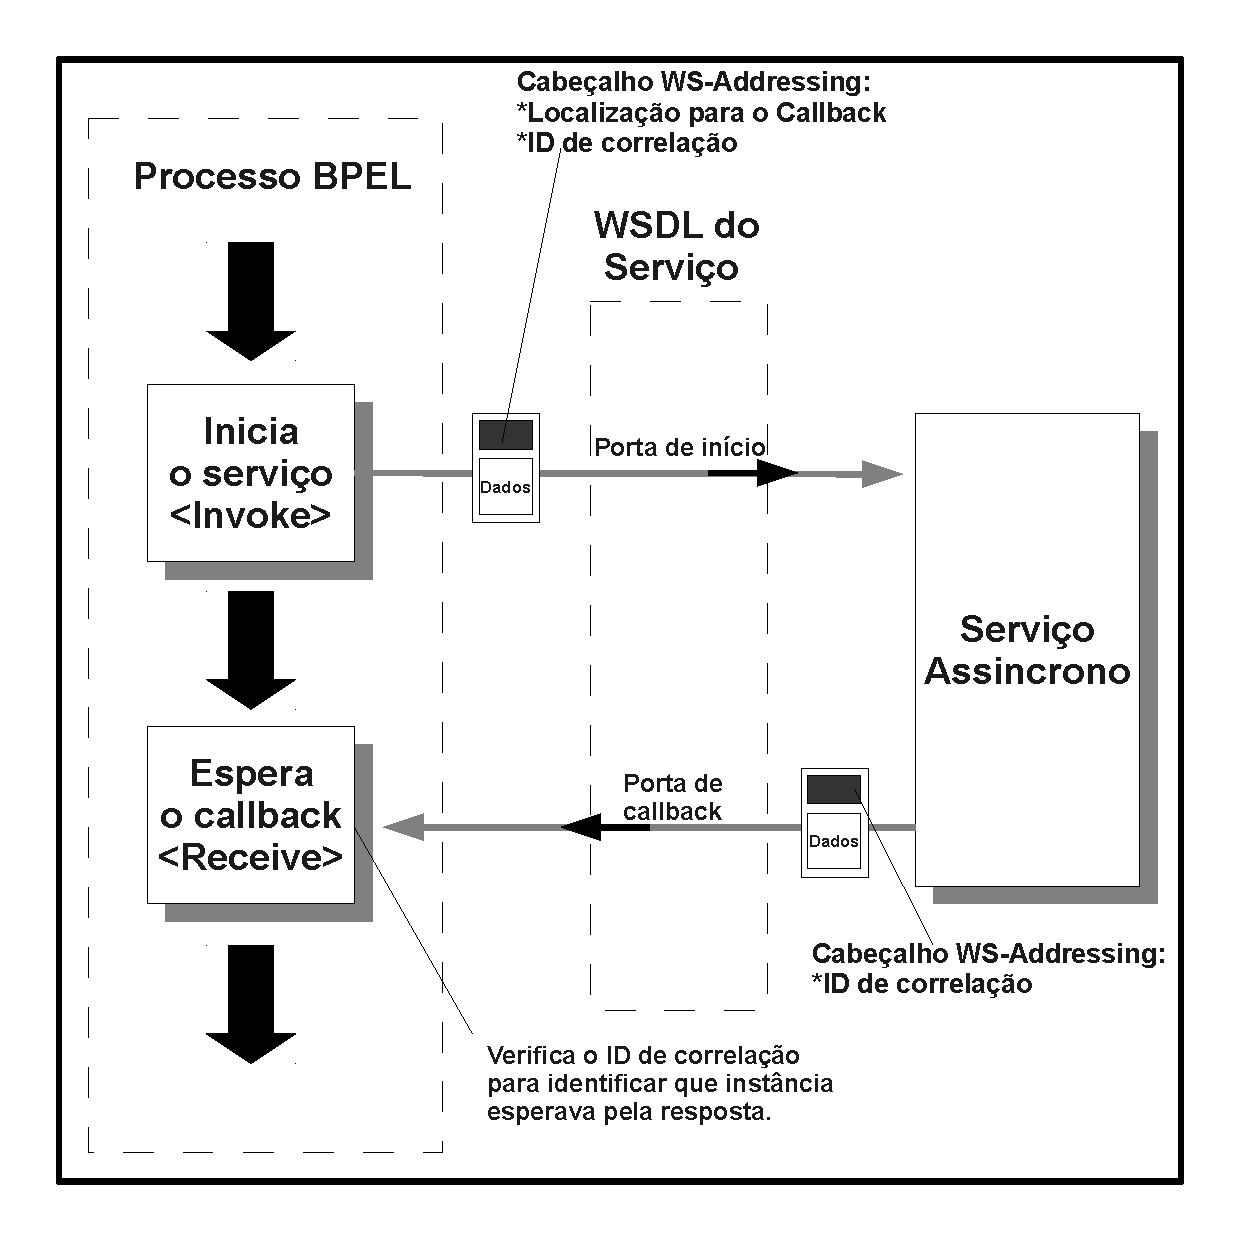
\includegraphics[scale=0.35]{imagens/bpelassinc.pdf}
			    %\caption{Processo WS-BPEL executando um WS de forma assíncrona.}
			\end{center}
		    \end{figure}		    
		    %\vspace{3cm} 
		\end{column}
		\begin{column}{5cm}
		\begin{overprint}
			\onslide<1>\textbf{1} - No BPEL, uma atividade \texttt{invoke} inicia um serviço (SOAP);
			\onslide<2>\textbf{2} - Cabeçalho WS-addressing é adicionado, informando o endereço do serviço para \textit{callback}, e o identificador de correlação;
			\onslide<3>\textbf{3} - Usando a descrição WSDL do serviço, uma porta é iniciada e os dados para o serviço assíncrono são enviados;
			\onslide<4>\textbf{4} - O serviço assíncrono processa a requisição e envia uma resposta de volta (porta de \textit{calback}).
			\onslide<5>\textbf{5} - O cabeçalho WS-addressing é montado com o identificador de correlação apropriado (o mesmo da mensagem \texttt{invoke});
			\onslide<6>\textbf{6} - A máquina de composição BPEL verifica o identificador de correlação e identifica a instância que aguardava.
		\end{overprint}
		\end{column}
	    \end{columns}	    	    
	\end{frame}
	
	\begin{frame}\frametitle{Execução de serviços assíncronos - BPEL}
	    Tempo de vida da chamada/resposta SOAP desacoplado do tempo de vida do protocolo HTTP, permitindo a execução de processos muito demorados.
	\end{frame}


\section{Trabalhos Relacionados}
    \begin{frame}
	\begin{center}
	{\Huge Trabalhos Relacionados}
	\end{center}
    \end{frame}
    \subsection{Execução de Workflows em Sistemas Distribuídos Heterogêneos}
	\begin{frame}\frametitle{Execução de WFs em Sistemas Distribuídos Heterogêneos}
	    \begin{table}[!htb]
		%\caption{Tabela comparativa de trabalhos correlatos (a).}
		\centering
		\small
		\begin{tabular}{l||c|c|c|c|c|c} % Define a quantidade de colunas
		    \hline
			\multirow{2}{2cm}{\textbf{Autor}} & \multicolumn{3}{c|}{\textbf{Arquitetura Alvo}} & \multicolumn{3}{c}{\textbf{Outras Propriedades}} \\
		    \cline{2-7}
			& \textbf{CoC} & \textbf{WSRF} & \textbf{OGSI} & \textbf{BPEL} & \textbf{Descoberta} & \textbf{Políticas} \\

		    \hline
		    \hline

		    Leymann  & Não & Não & Não & Sim & Não & Não \\ 
		    Slomiski & Não & Sim & Sim & Sim & Não & Não \\
		    Emmerich & Não & Não & Sim & Sim & Não & Não \\
		    Ezenwoye & Não & Sim & Não & Sim & Sim & Não \\
		    Ma 	     & Não & Sim & Não & Sim & Não & Não \\
		    \textbf{Lechuga} & \textbf{Sim} & \textbf{Não} & \textbf{Não} & \textbf{Sim} & \textbf{Sim} & \textbf{Sim} \\ 

		    \hline
		\end{tabular}
	    \end{table}
	\end{frame}
	
    \subsection{Escalonamento Global em Clusters de Clusters}
	\begin{frame}\frametitle{Escalonamento Global em CoCs}
	    \begin{table}[!htb]
		%\caption{Tabela comparativa de trabalhos correlatos (b).}
		\centering
		\small
		\begin{tabular}{l||c|c|c|c} % Define a quantidade de colunas
		    \hline
		    \multirow{2}{2cm}{\textbf{Autor}} & \multicolumn{2}{c|}{\textbf{Problemas}} & \multicolumn{2}{c}{\textbf{Vantagens}} \\
		    \cline{2-5}
		    & \textbf{Central.} & \textbf{Alterações} & \textbf{Implement.} & \textbf{Compatib.} \\

		    \hline
		    \hline

		    Chau     & Não & Sim & Não & Não \\ 
		    Takpé    & Sim & Não & Não & Não \\
		    Qin	     & Sim & Sim & Não & Não \\
		    Hunold   & Não & Não & Não & Não \\
		    Beltrán  & Não & Sim & Sim & Não \\
		    \textbf{Lechuga} & \textbf{Não} & \textbf{Não} & \textbf{Sim} & \textbf{Sim} \\ 

		    \hline
		\end{tabular}
	    \end{table}
	\end{frame}
    
\section{Infraestrutura para a Execução de WFs em CoCs}
    \begin{frame}
	\begin{center}
	{\Huge Infraestrutura para a Execução de WFs em CoCs}
	\end{center}
    \end{frame}
    
    \subsection{Estendendo o WS-BPEL para especificação de QoS}
	\begin{frame} \frametitle{Estendendo o WS-BPEL para especificação de QoS}
	    \begin{itemize}
		\item Seleção de serviços baseada em especificações de QoS e Recursos.
		    \begin{itemize}
			\item Inclusão de informações de recursos requeridos para a execução.
			    \note[item] {Serviços podem ter necessidades relacionadas a aspectos como poder de processamento, capacidade de memória e disco.}
			\item Requisitos dos usuários e capacidade dos provedores.			
		    \end{itemize}
		\item Informações de QoS especificadas como políticas em WS-Policy e armazenadas em um repositório.
		\item Funcionalidades e atributos de QoS em arquivos separados (WS-PolicyAttachment).
	    \end{itemize}
	\end{frame}
	
	\begin{frame}[fragile]\frametitle{Estendendo o WS-BPEL para especificação de QoS}
	    %Exemplo SOAP
 		\begin{figure}[!htb]
 		    \centering
		    \lstinputlisting[basicstyle=\tiny]{listings/policy-bpel.xml}
 		\caption{Exemplo de política em uma composição de serviços.}
 		\end{figure}
	\end{frame}
    
    \subsection{Proposta de Arquitetura}
	\begin{frame} \frametitle{Proposta de Arquitetura}
	\note[item] {Para ganhar tempo, vou explicar com detalhes na aplicada.}
	    \begin{itemize}
		\item Todas as funcionalidades adicionais em uma nova camada.
	    \end{itemize}
	    \begin{center}
		\begin{figure}
		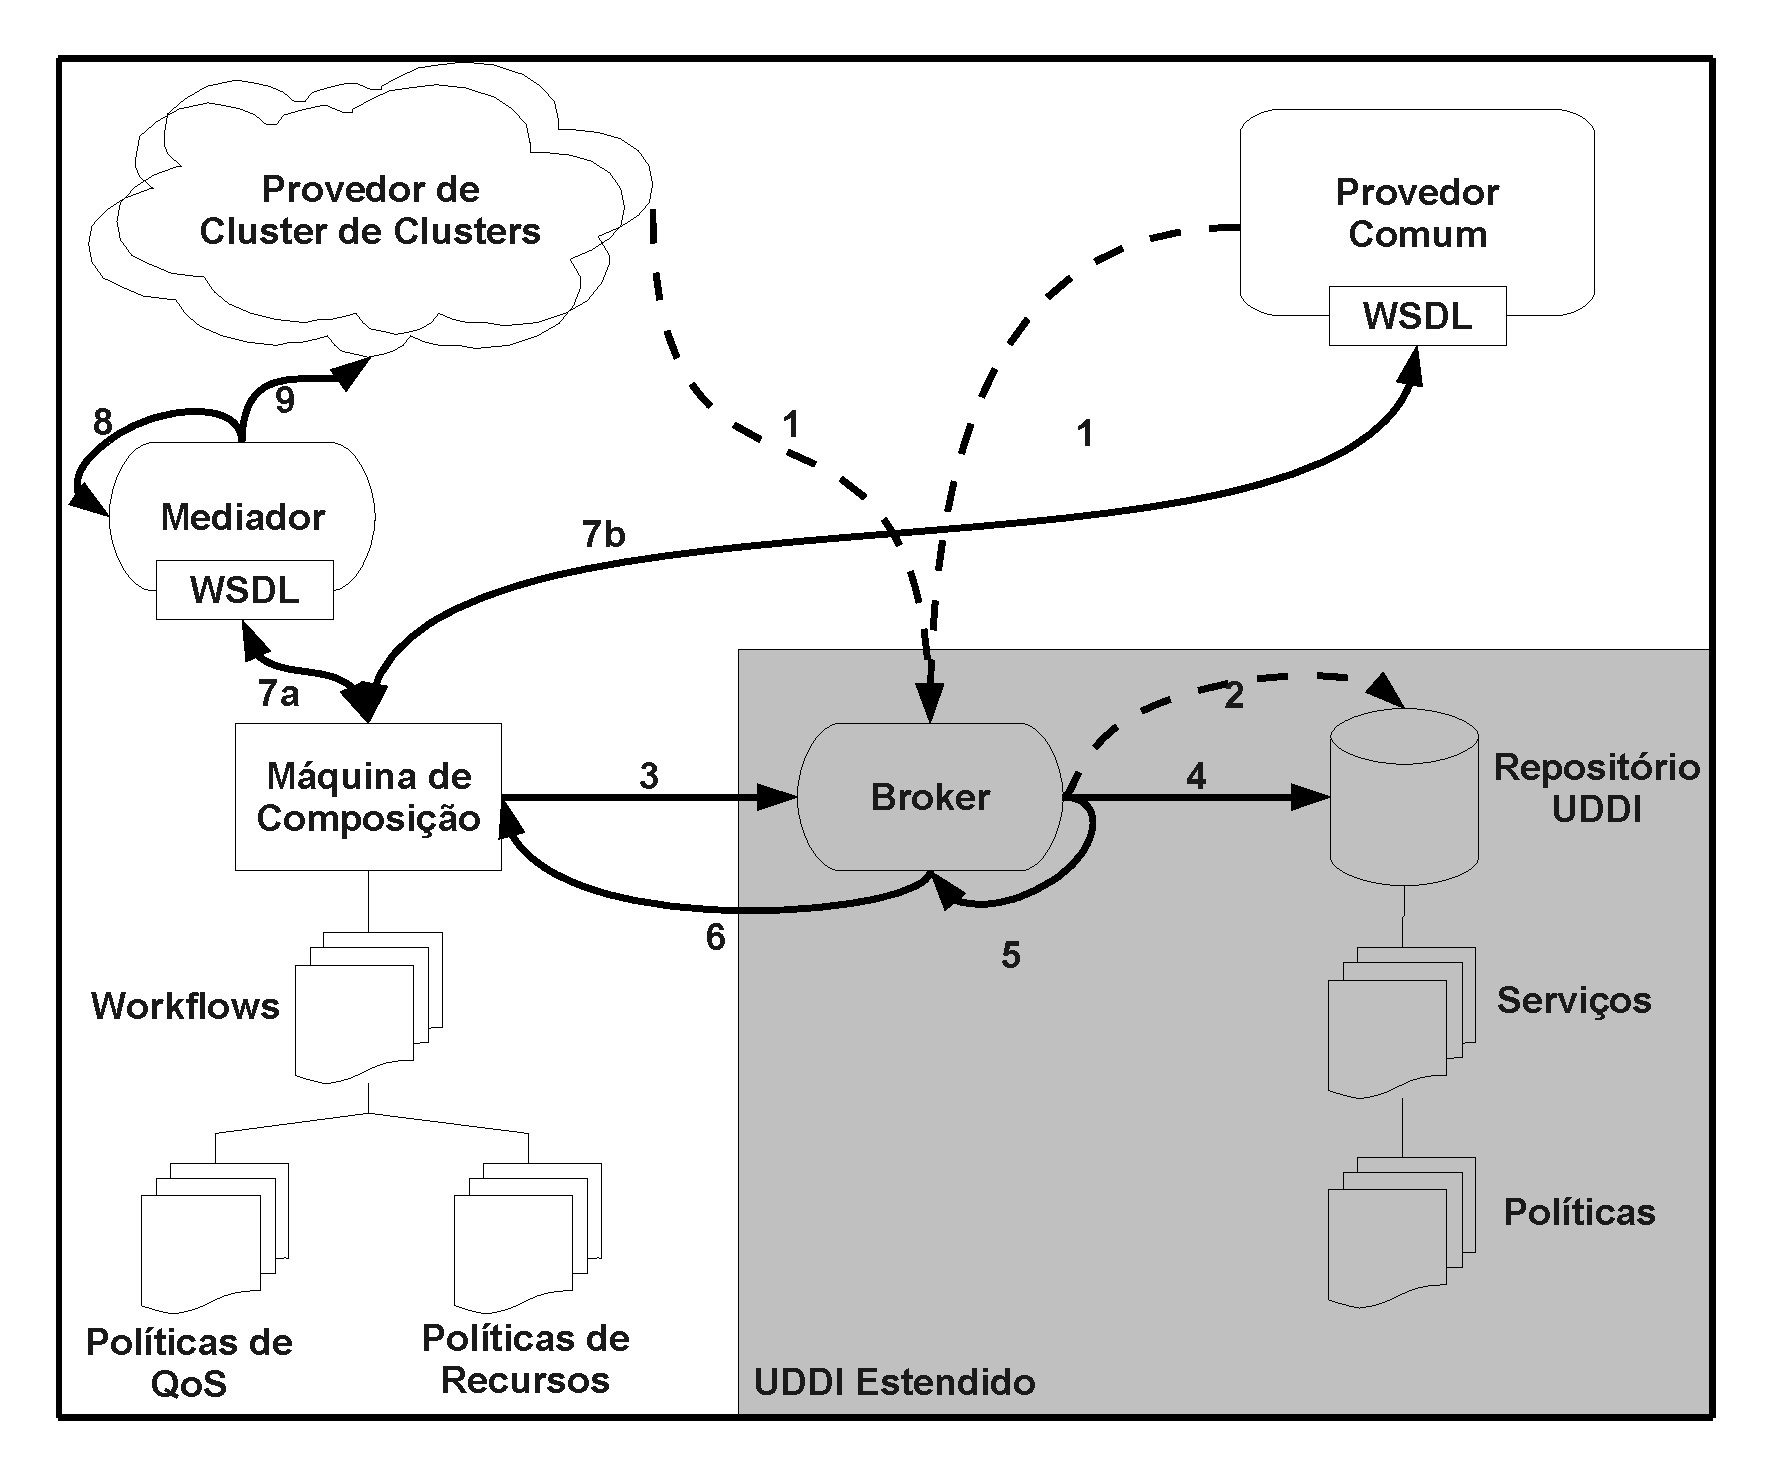
\includegraphics[scale=0.24]{imagens/execComposicaoG.pdf}		
		\end{figure}
	    \end{center}
	\end{frame}
    
    
\section{Estudo de Caso: SHARCNET}
    \begin{frame}
	\begin{center}
	{\Huge Estudo de caso: SHARCNET}
	\end{center}
    \end{frame}
    \subsection{A SHARCNET}
	\begin{frame} \frametitle{A SHARCNET}
	    \begin{itemize}
		\item Rede multi-institucional de \textit{clusters} de alta performance.
		\item Distribuídos em dezesseis instituições acadêmicas na província de Ontário, no Canadá.
		\item Ausência de escalonador global.
		    \begin{itemize}
			\item ``Impossibilidade'' de execução automatizada. Workflow!
		    \end{itemize}
	    \end{itemize}
	\end{frame}
    
    \subsection{Arquitetura Aplicada}    
	\begin{frame} \frametitle{Arquitetura Aplicada}
	    \begin{center}
		\begin{figure}
		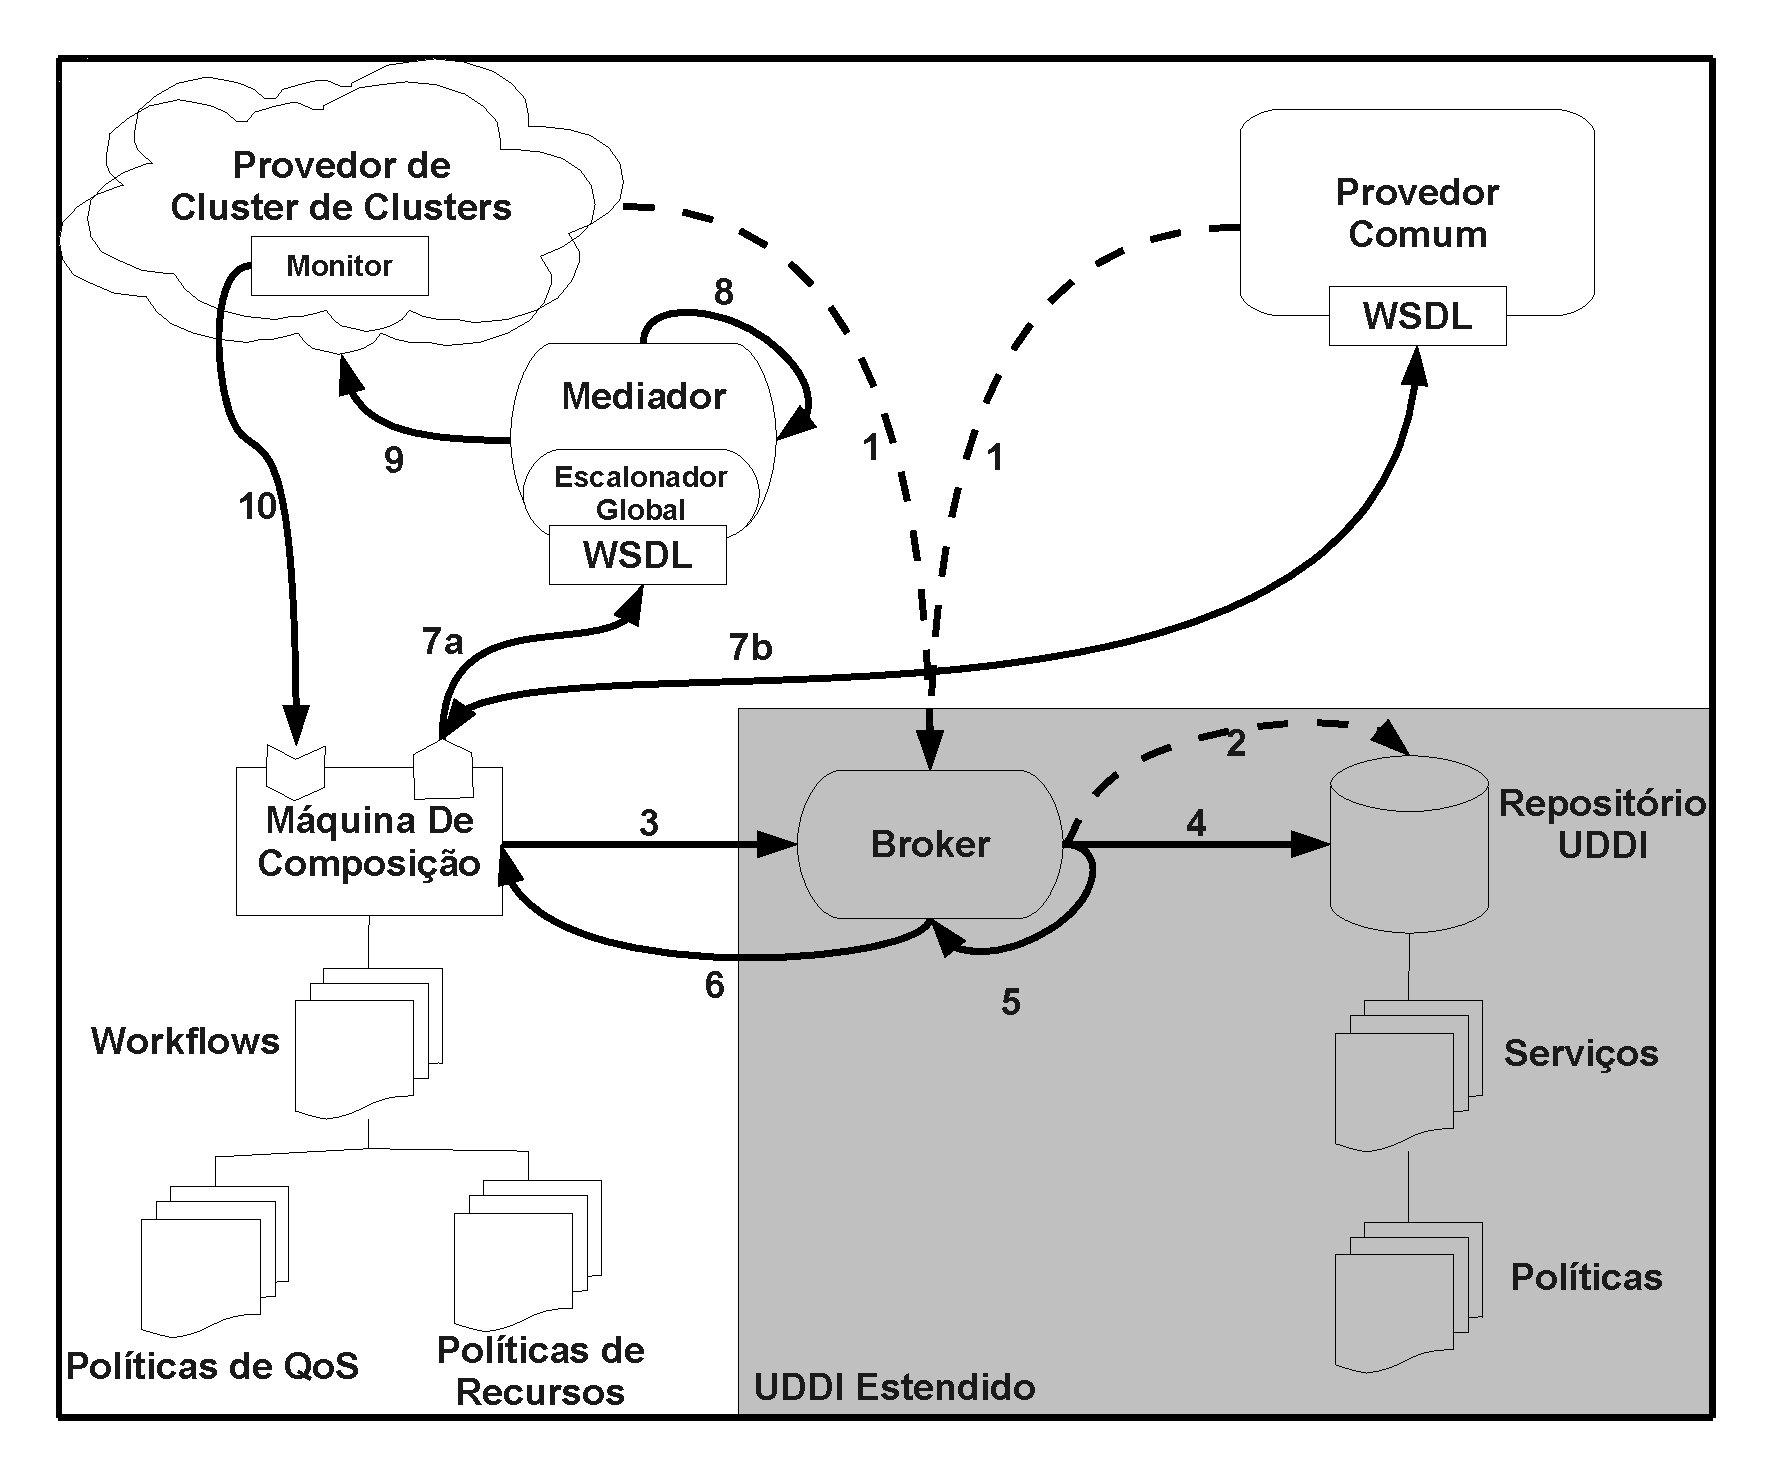
\includegraphics[scale=0.25]{imagens/execComposicaoA.pdf}	    
		\end{figure}
	    \end{center}
	\end{frame}
	
	\begin{frame} \frametitle{Máquina de Composição}
	    \begin{center}
		\begin{figure}
		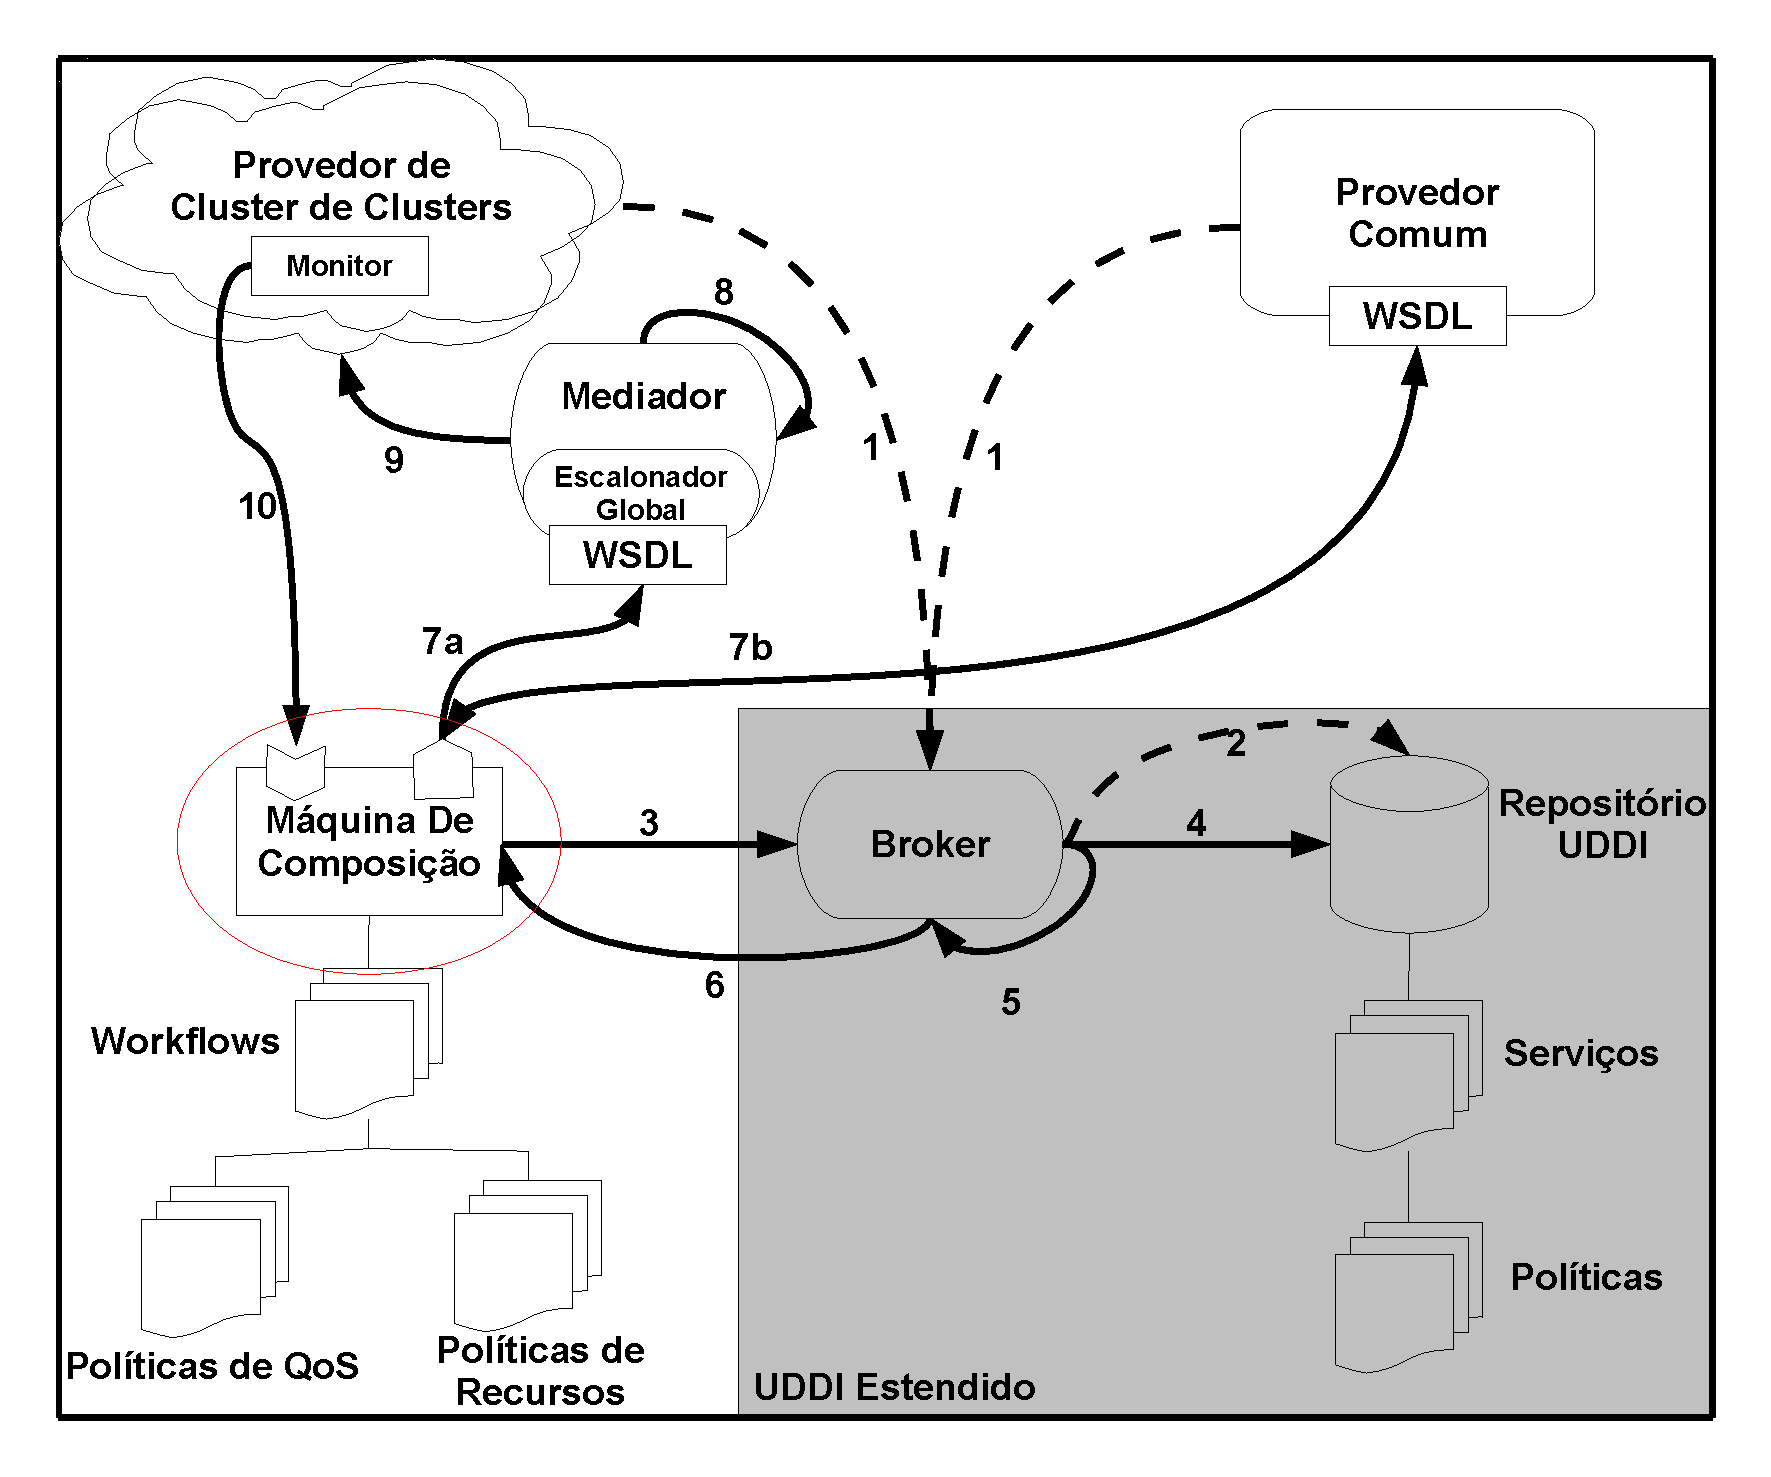
\includegraphics[scale=0.25]{imagens/execComposicaoA-1.pdf}	    
		\end{figure}
	    \end{center}
	\end{frame}
	
	\begin{frame} \frametitle{Máquina de Composição}
	    \begin{itemize}
		\item Componente mais importante para a execução de um processo BPEL.
		\item \textit{BPEL Service Engine} para Glasfish Open ESB no Netbeans.
		\item Arquitetura adaptada para funcionalidades padrão do componente.
		\item Não foi modificada. 
	    \end{itemize}	
	\end{frame}
	
	\begin{frame} \frametitle{Broker}
	    \begin{center}
		\begin{figure}
		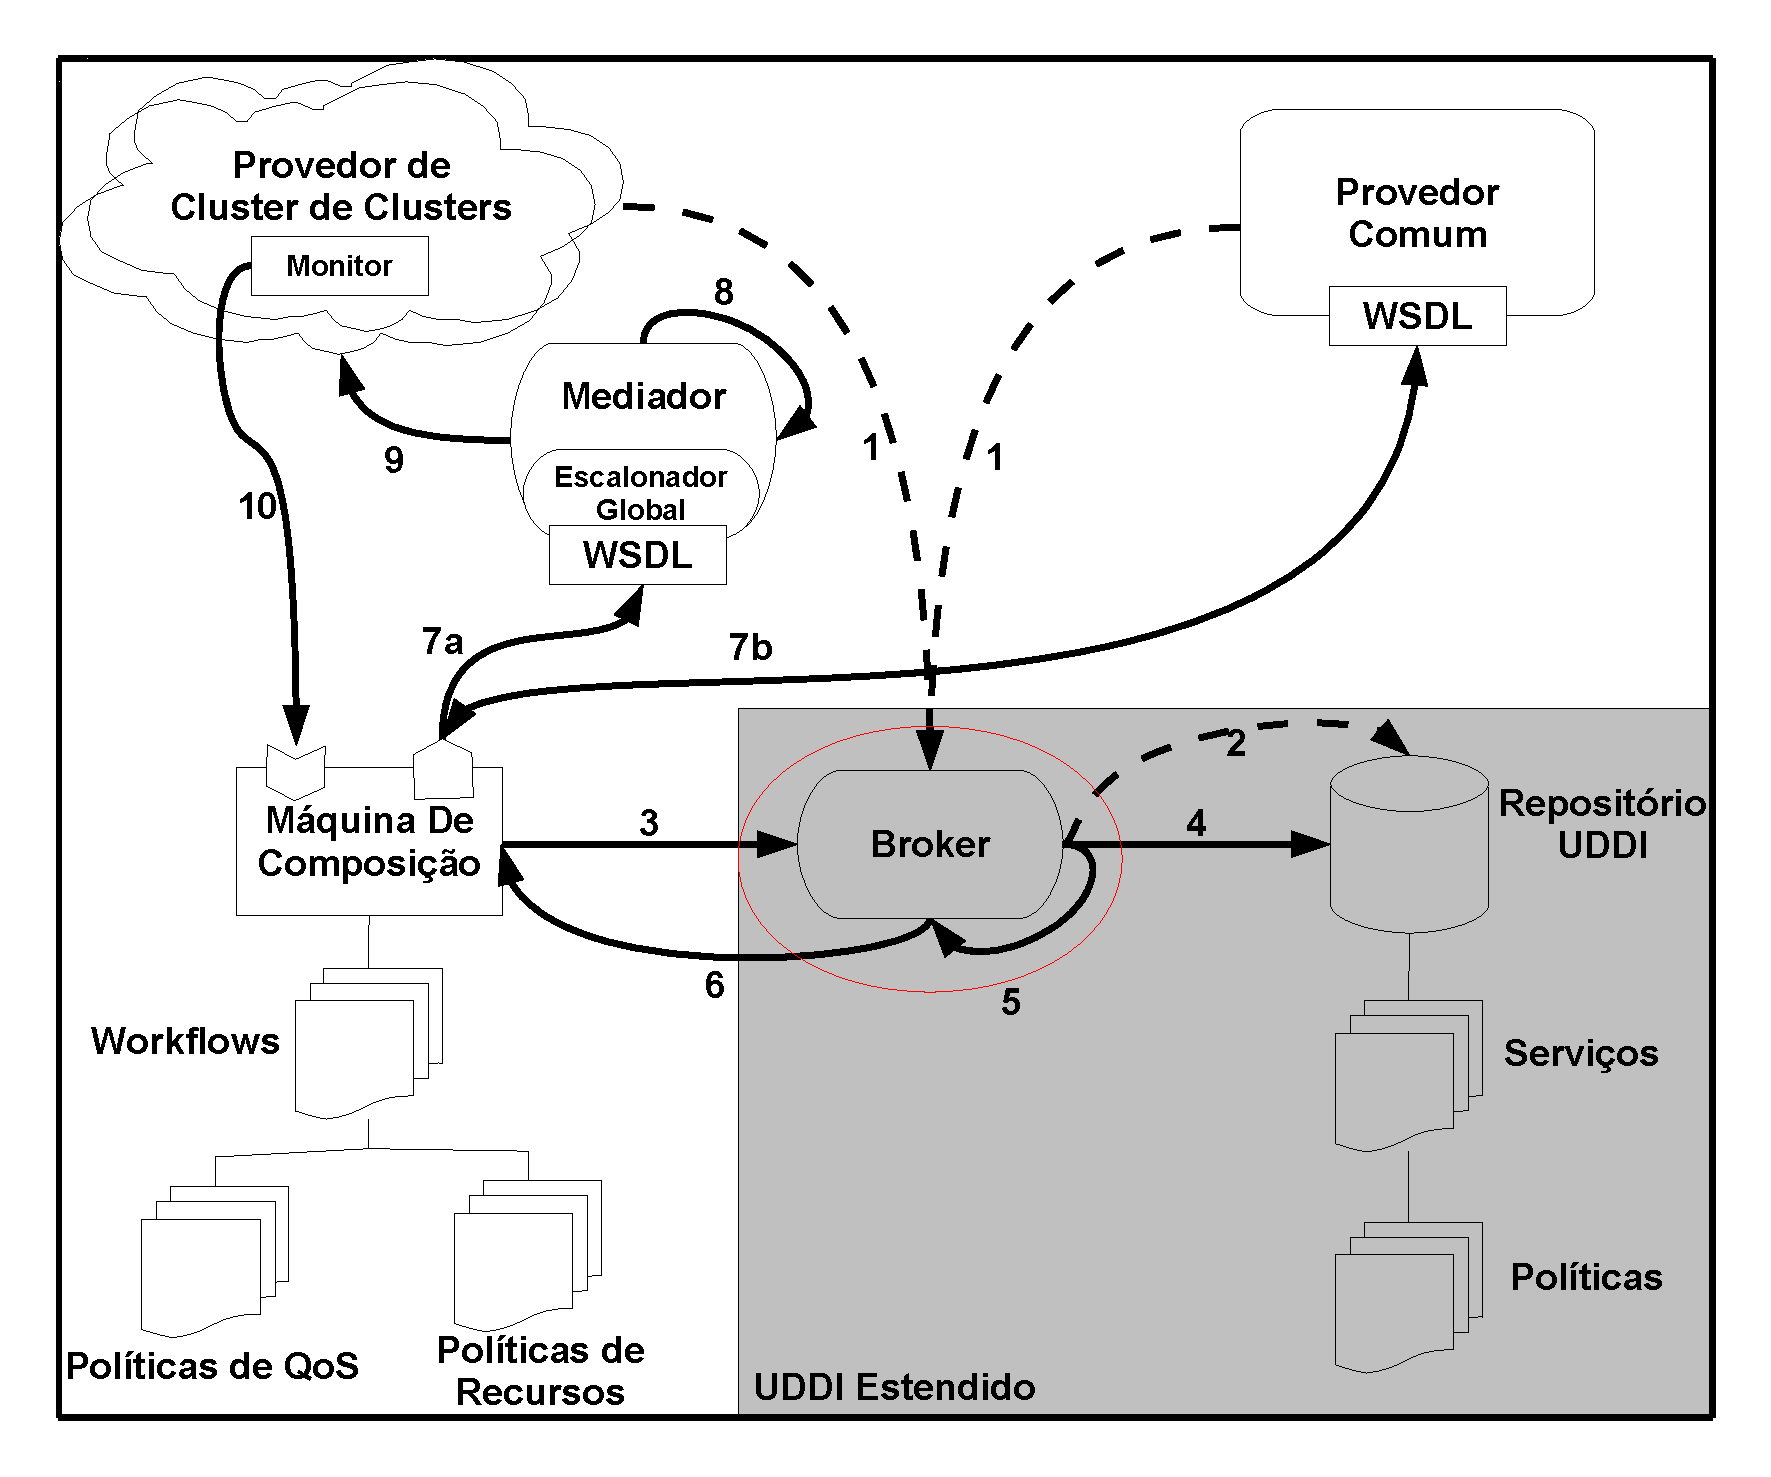
\includegraphics[scale=0.25]{imagens/execComposicaoA-2.pdf}	    
		\end{figure}
	    \end{center}
	\end{frame}

	\begin{frame} \frametitle{Broker}
	    \begin{itemize}
		\item Parte principal do UDDI estendido proposto por Garcia e Toledo.
		\item WS de interface para um UDDI.
		\item Busca por requisitos funcionais e de QoS.
		\item Retorna o serviço mais indicado.
		\item \textit{Binding} Dinâmico.
	    \end{itemize}				
	\end{frame}

	\begin{frame} \frametitle{UDDI}
	    \begin{center}
		\begin{figure}
		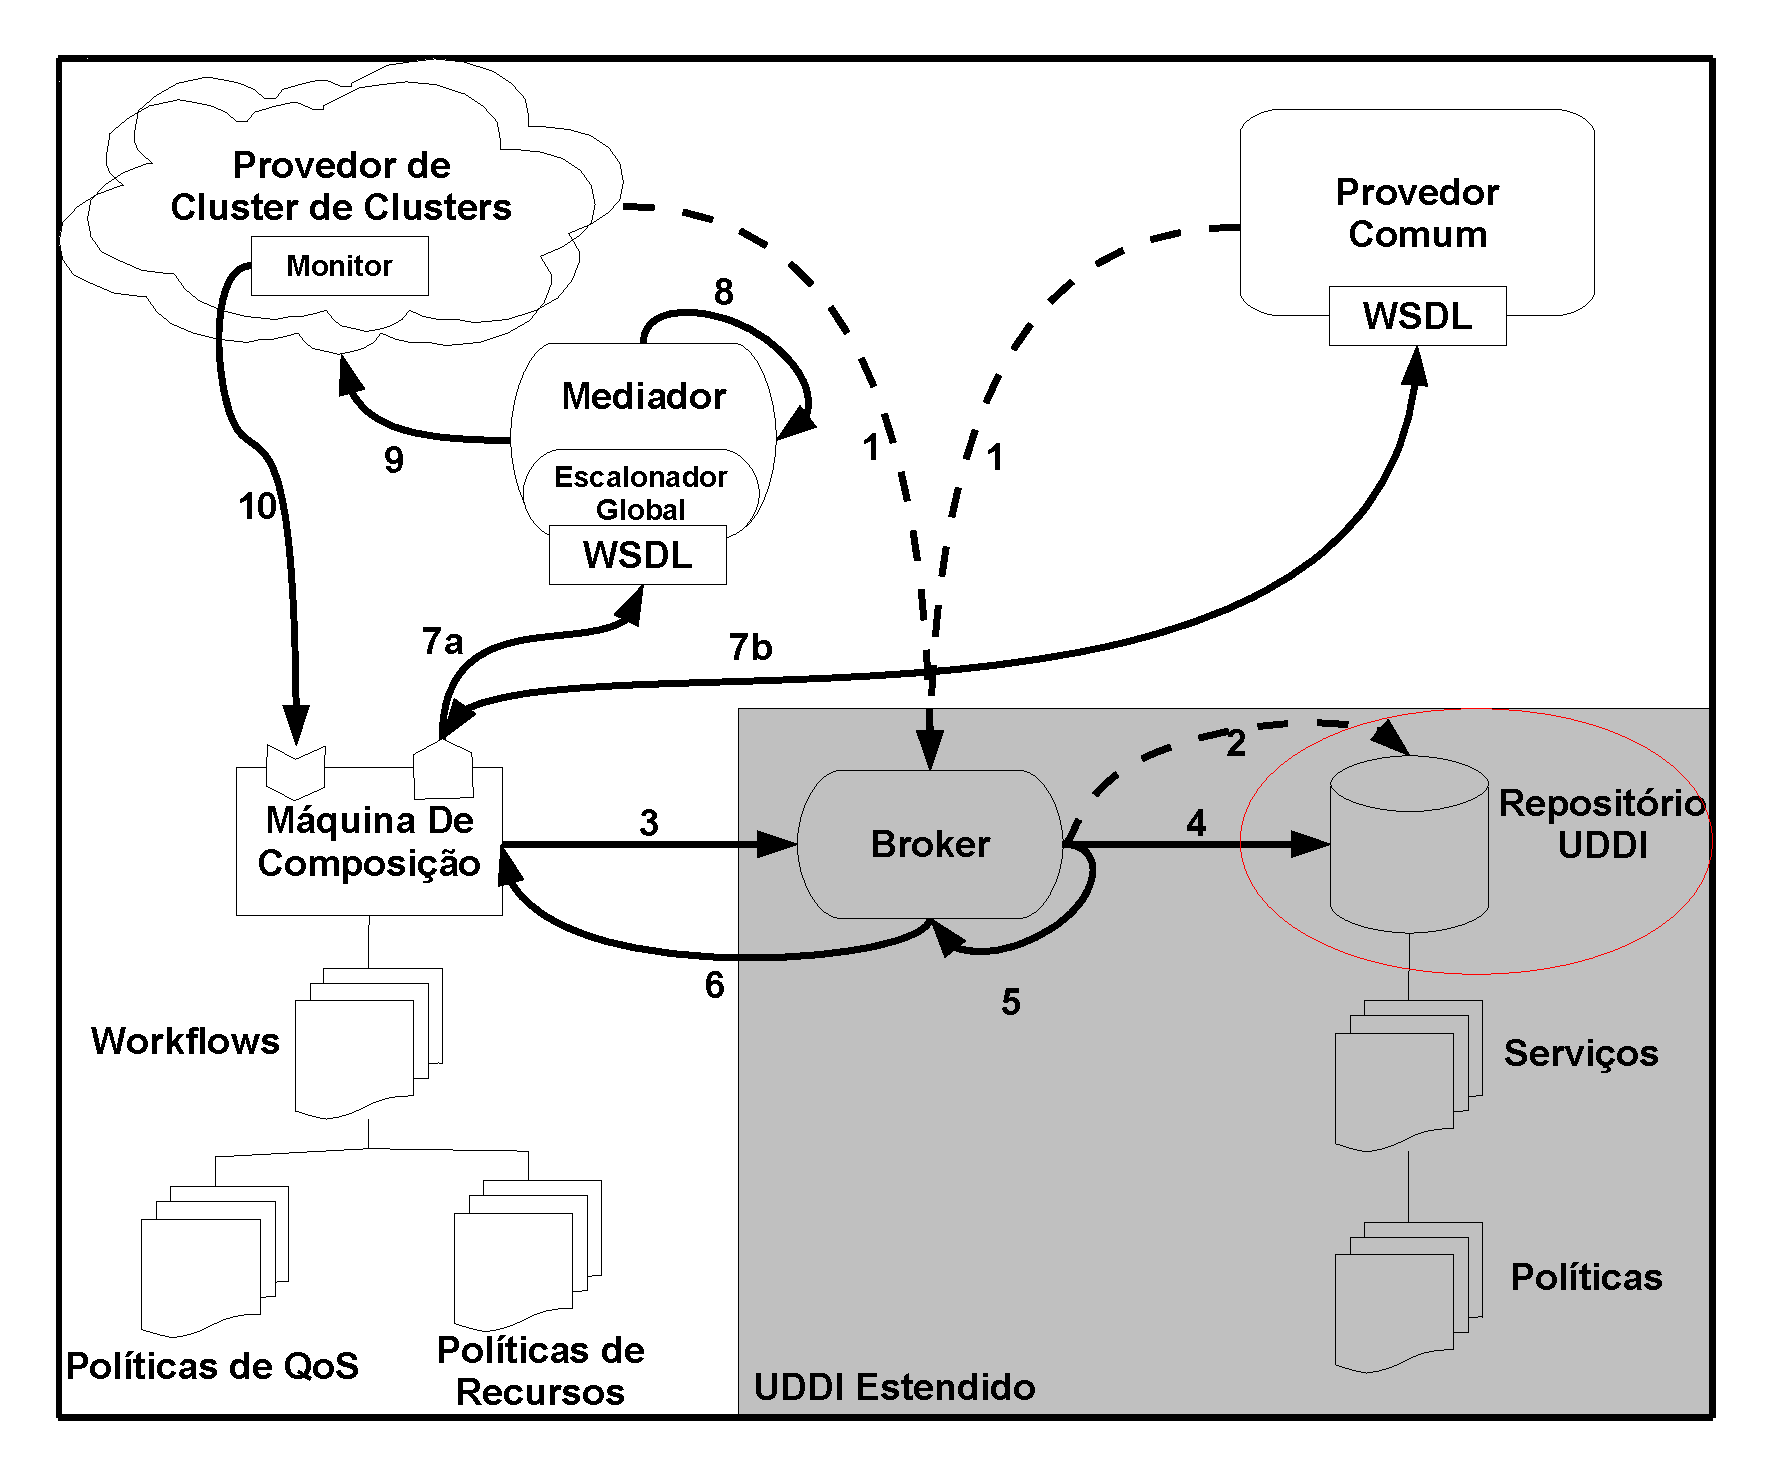
\includegraphics[scale=0.25]{imagens/execComposicaoA-3.pdf}	    
		\end{figure}
	    \end{center}
	\end{frame}
	
	\begin{frame} \frametitle{UDDI}
	    \begin{itemize}
		\item Armazenar os serviços publicados e auxiliar o \texttt{Broker} nas buscas.
		\item JUDDI.
	    \end{itemize}
	\end{frame}
	
	\begin{frame} \frametitle{Mediador}
	    \begin{center}
		\begin{figure}
		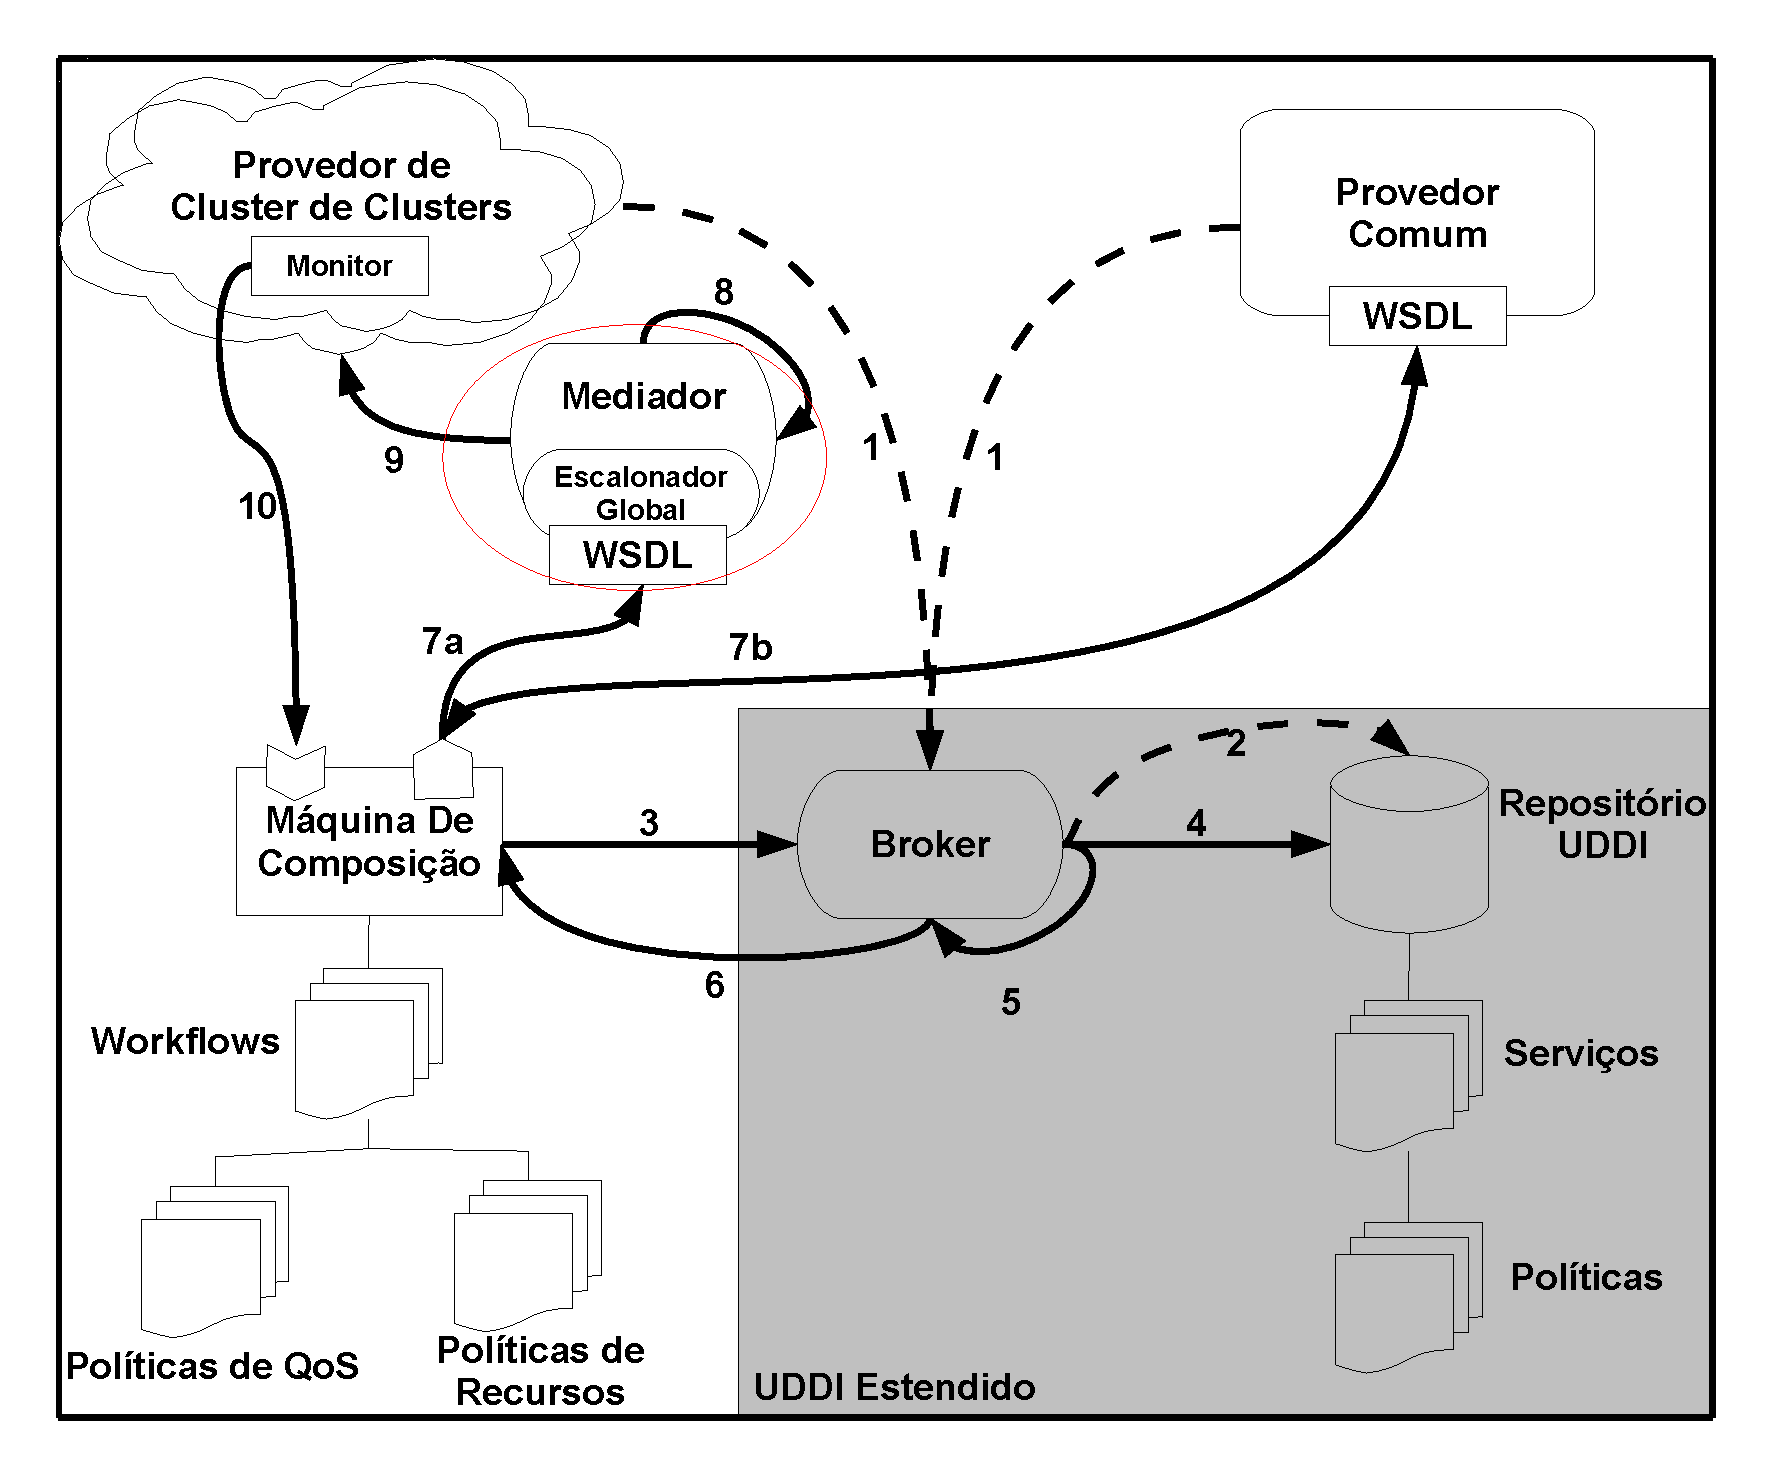
\includegraphics[scale=0.25]{imagens/execComposicaoA-4.pdf}	    
		\end{figure}
	    \end{center}
	\end{frame}

	\begin{frame} \frametitle{Mediador}
	    \begin{itemize}
		\item WS que atua como um \textit{proxy} para a SHARCNET.
		    \note[item] {fazendo a interface entre a \texttt{Máquina de Composição} e a SHARCNET. Todas as requisições direcionadas a ela devem ser enviadas ao \texttt{Mediador}}
		    \note[item] {Responsável por gerenciar a execução das tarefas.}
		\item Verifica os requisitos (descritos nas políticas) e invoca os outros componentes da arquitetura.
		\item Não é centralizado.
		\item Invocação assíncrona.
		    \note[item] {Não envia a resposta. -- Monitor}
	    \end{itemize}
	\end{frame}
	
	\begin{frame} \frametitle{Escalonador Global}
	    \begin{center}
		\begin{figure}
		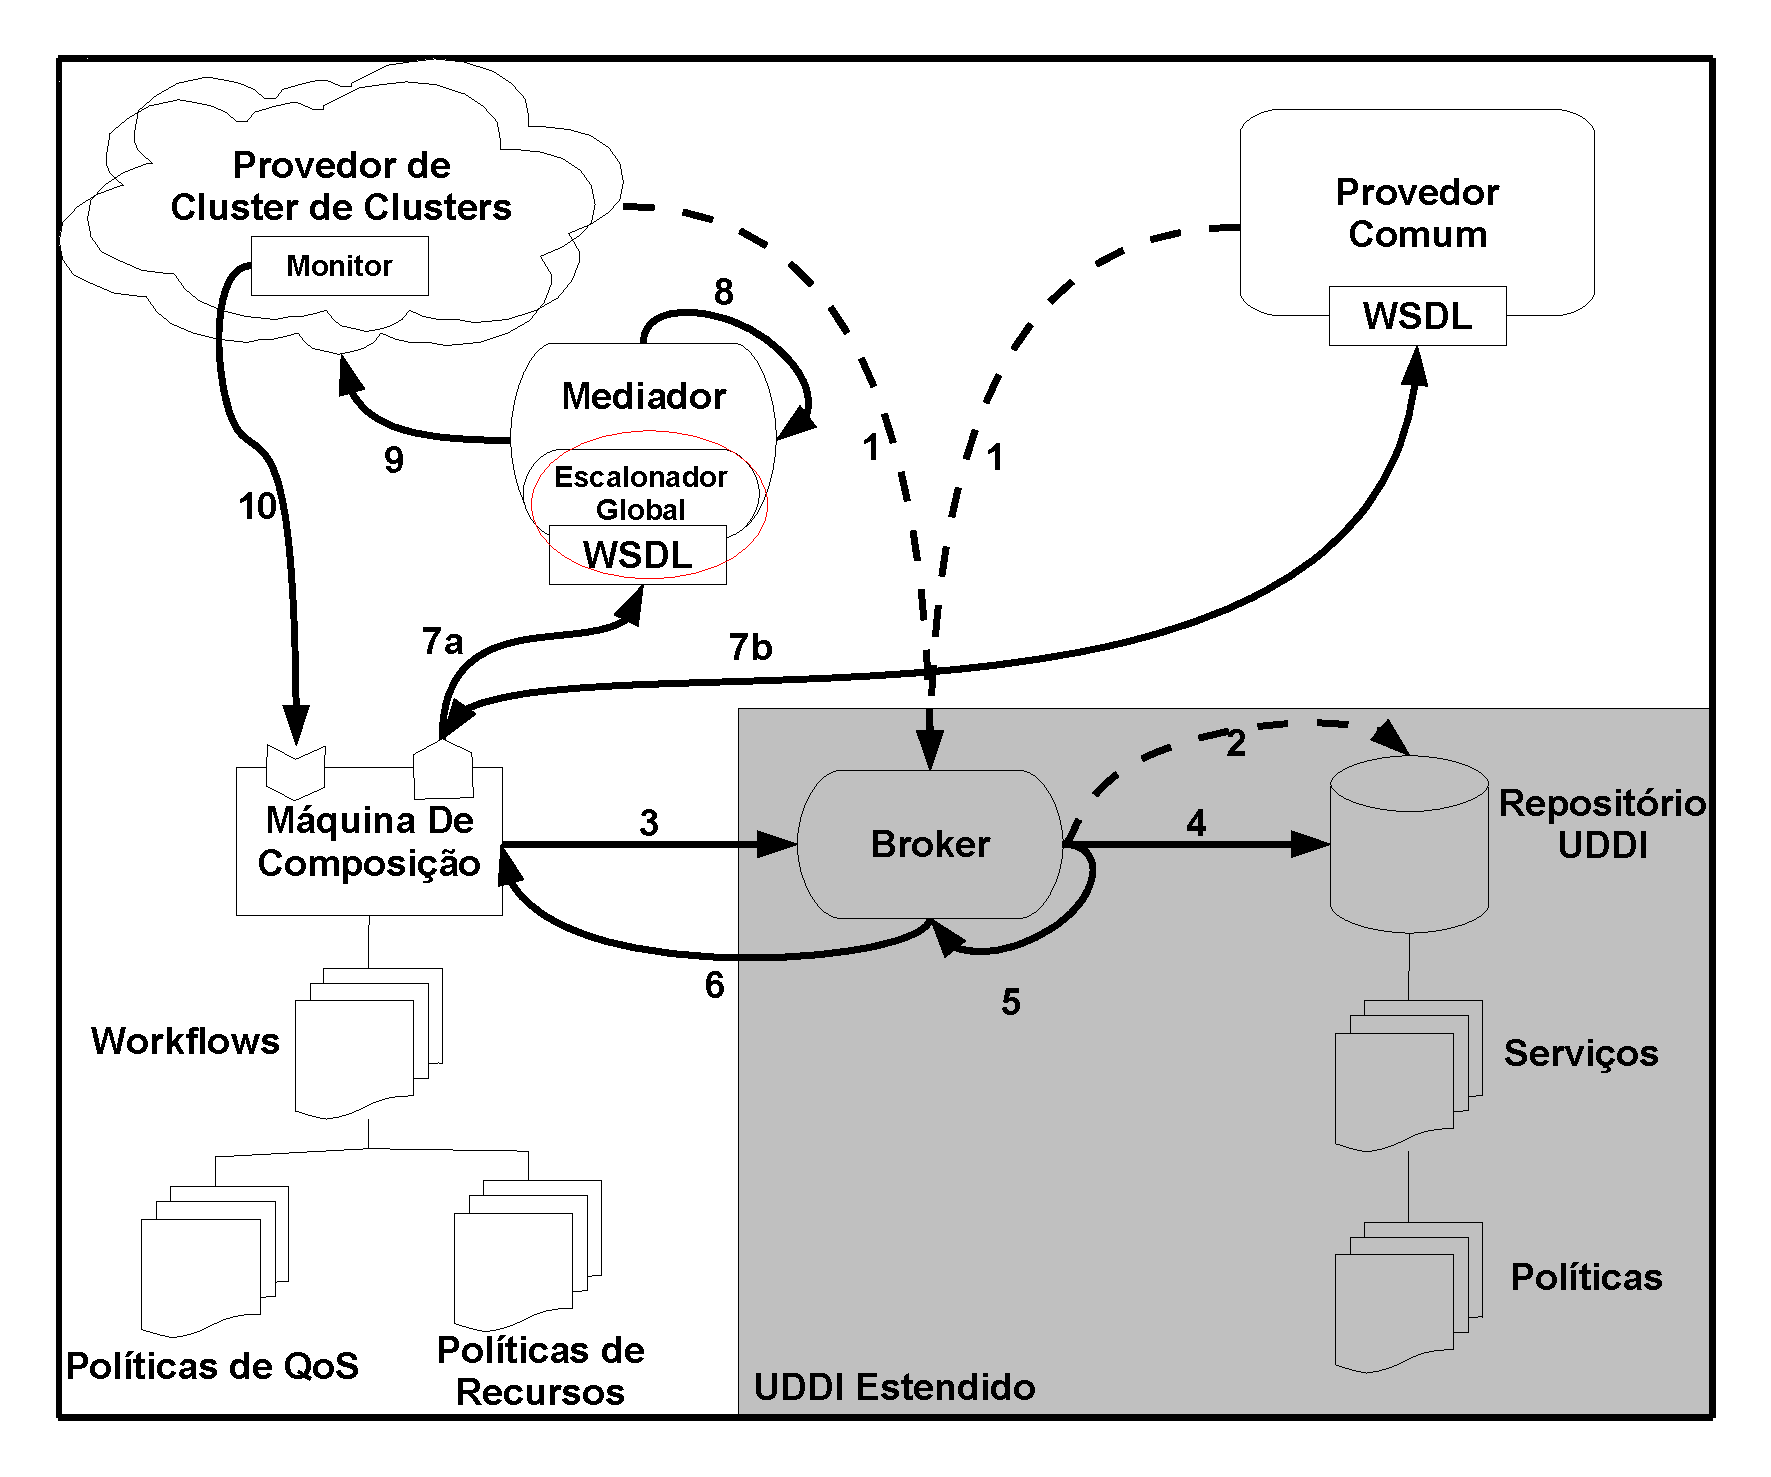
\includegraphics[scale=0.25]{imagens/execComposicaoA-5.pdf}	    
		\end{figure}
	    \end{center}
	\end{frame}

	\begin{frame} \frametitle{Escalonador Global}
	    \begin{itemize}
		\item Parceria com a UWO.
		\item Compatibilidade com a seleção manual de recursos: Aplicações existentes não são modificadas.
		\item Cenário:
	    \end{itemize}
	    \begin{center}
		\begin{figure}
		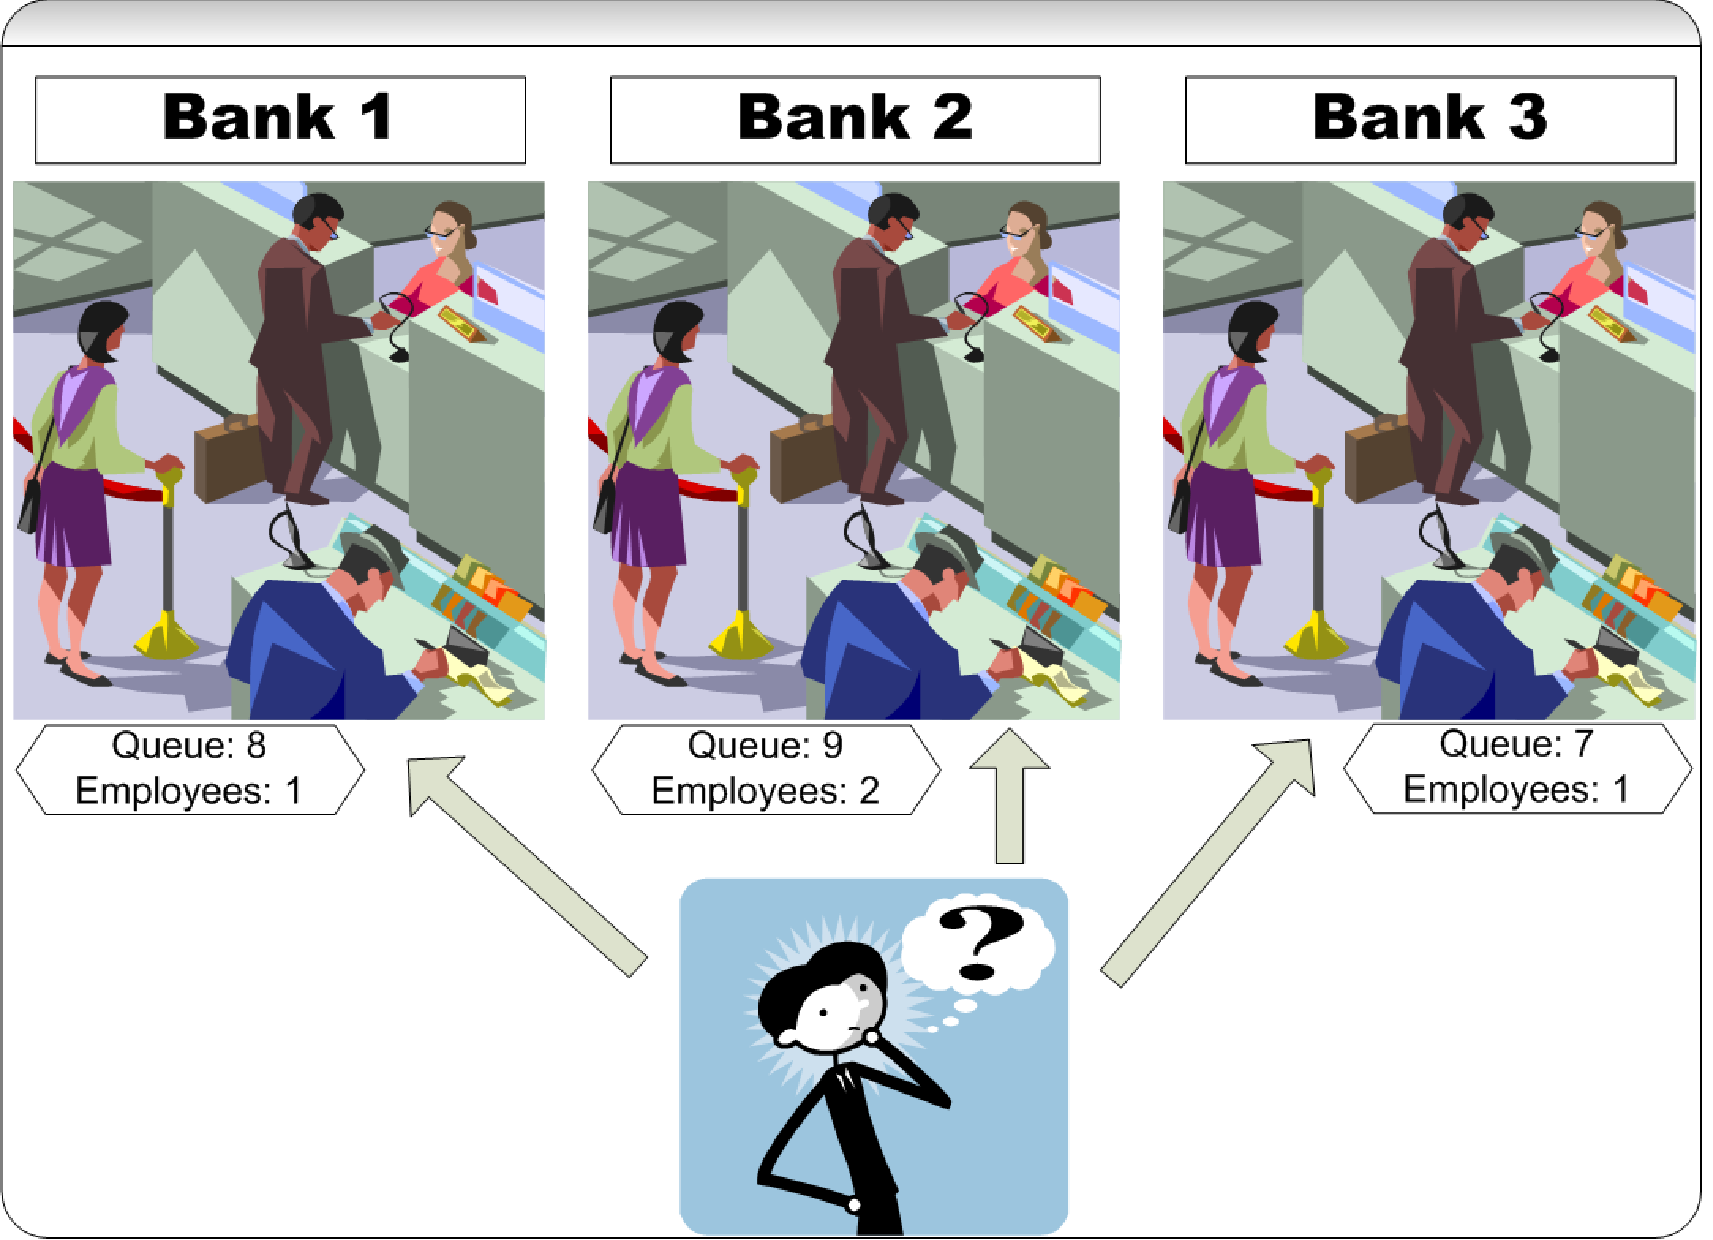
\includegraphics[scale=0.15]{imagens/banco.pdf}
		\caption{Fila de Banco}
		\end{figure}
	    \end{center}
	\end{frame}

	\begin{frame} \frametitle{Escalonador Global}
	    \begin{itemize}
		\item Métrica proposta para comparar a carga de cada HPCC:
	    \end{itemize}
	    \begin{block}{Formula}
		\begin{center}
		$\frac{Quantidade\; de\; processadores\; requisitados\; pela\; fila}{Quantidade\; total\; de\;  processadores * Potencia\; dos\; processadores}$
		\end{center}
	    \end{block}
	    \begin{itemize}		
		\item Envia a tarefa para o \textit{cluster} que melhor atende os requisitos.
		\item Método simples e distribuído.
	    \end{itemize}
	    \begin{center}
		\begin{figure}
		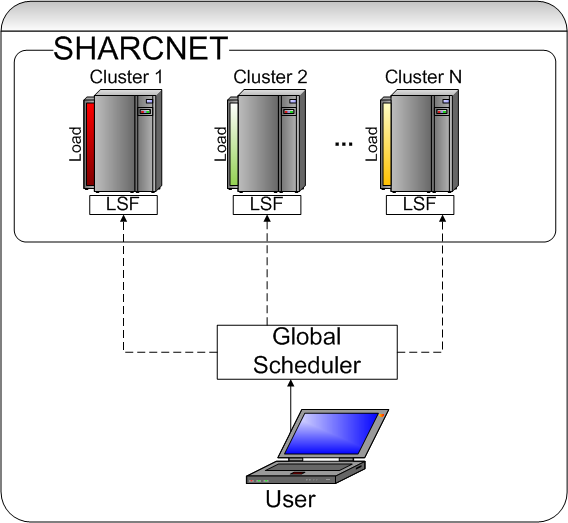
\includegraphics[scale=0.15]{imagens/scheduler.png}
		\caption{Arquitetura do Escalonador}
		\end{figure}
	    \end{center}
	\end{frame}
	
	\begin{frame} \frametitle{Monitor}
	    \begin{center}
		\begin{figure}
		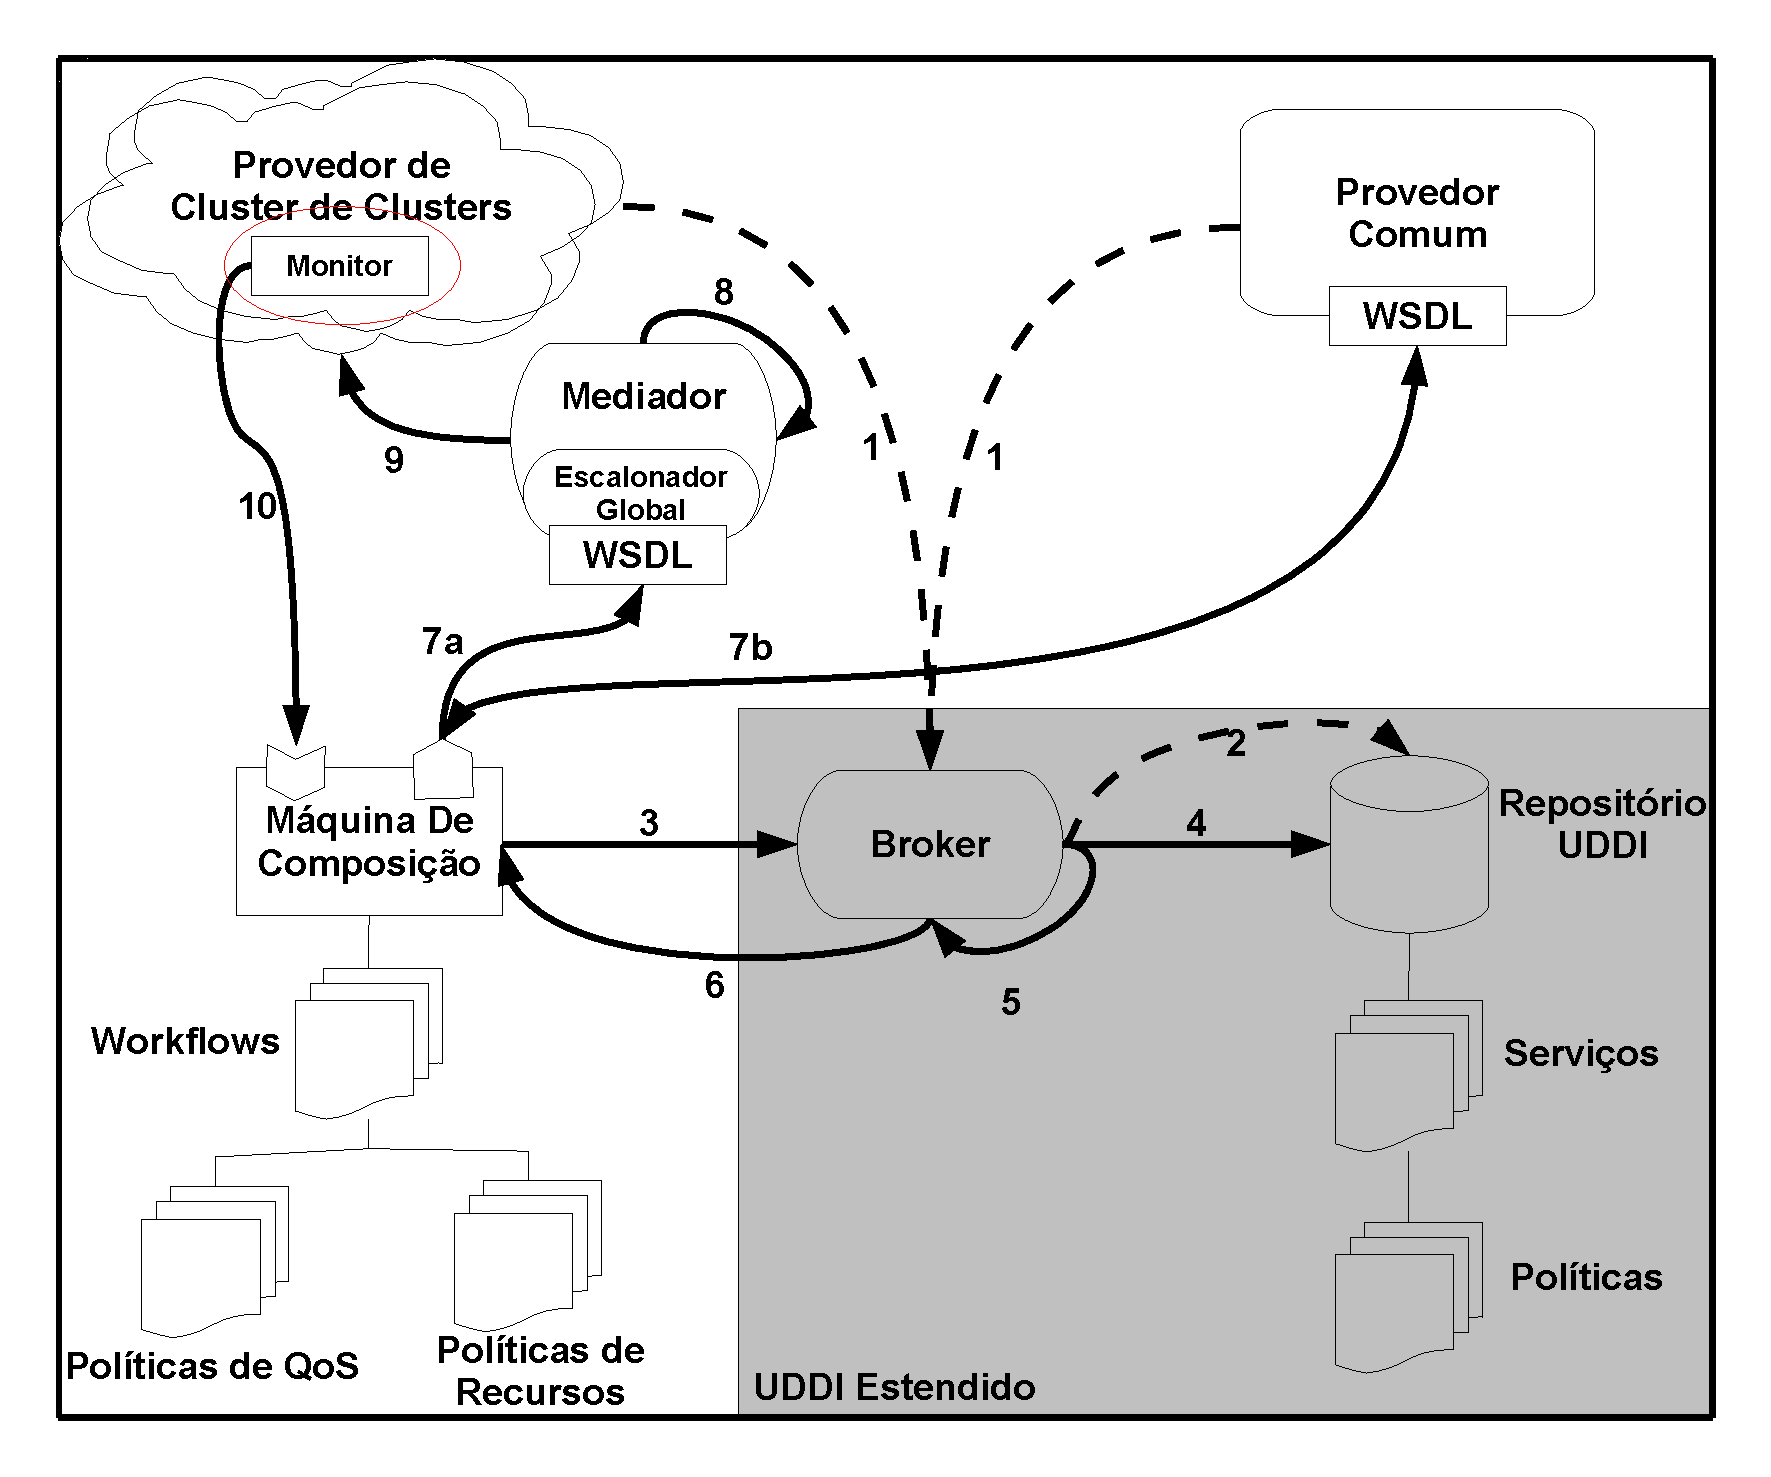
\includegraphics[scale=0.25]{imagens/execComposicaoA-6.pdf}    
		\end{figure}
	    \end{center}
	\end{frame}
	
	\begin{frame} \frametitle{Monitor}
	    \begin{itemize}
		\item Monitora o estado dos serviços sendo executados na SHARCNET.
		\item Uma instância por tarefa.
		\item Quando a tarefa é concluída, lê o resultado e envia a resposta para o endereço de \textit{callback} (WS-Addressing).
	    \end{itemize}
	\end{frame}        

    
\section{Aplicação}
    \begin{frame}
	\begin{center}
	{\Huge Aplicação}
	\end{center}
    \end{frame}
    
    \subsection{Montage}
	\begin{frame} \frametitle{Montage}
	    \begin{itemize}
		\item Conjunto de ferramentas criadas pela NASA para gerar mosaicos personalizados do céu (WF).
		\item Entrada FITS (Sistema de Transporte Imagem Flexível).
		\item Reprojetar imagens, gerar mosaico inicial, modelar planos de fundo, combinar planos de fundo, e gerar mosaico corrigido.
		\item Dez imagens do Atlas 2MASS da galáxia Pinwheel, ou M101.
	    \end{itemize}
	\end{frame}  
    
    \subsection{Implementação}
	\begin{frame} \frametitle{Implementação}
	    \begin{itemize}
		\item Seis Serviços Web:
		    \begin{itemize}
			\item Um para cada etapa do algoritmo;
			\item Extra para transferência de dados.
		    \end{itemize}
		\item Interação descrita com WS-BPEL.
		\item Etapa 1 (Reprojeção) executada na SHARCNET.
	    \end{itemize}
	\end{frame}
	
	\begin{frame}[plain]\frametitle{BPEL}
	    \begin{figure}[!htb]%Figura:Imagem BPEL M101
		\begin{center}
		    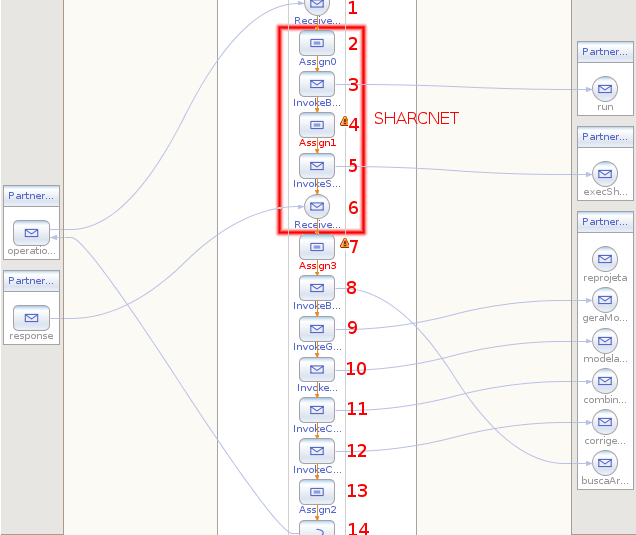
\includegraphics[scale=0.4]{imagens/ImM101BPEL.png}   
		\end{center}
	    \end{figure}
	    	    
	    \note[item] {Recebe a chamada de inicio e começa a execução.}
	    \note[item] {Parâmetros para a chamada ao UDDI Ext. são configurados.}
	    \note[item] {O UDDI Ext. é consultado (retornar o URI para a SHARCNET).}
	    \note[item] {Configura chamada para exec SHARCNET.}
	    \note[item] {Etapa do algoritmo Montage é executada na SHARCNET.}
	    \note[item] {A SHARCNET envia a resposta de forma assíncrona.}
	    \note[item] {Os parâmetros para o restante do WF são configurados.}
	    \note[item] {O serviço para executar a transferência de arquivos.}
	    \note[item] {O serviço com a segunda etapa do Montage é invocado.}
	    \note[item] {O serviço com a terceira etapa do Montage é invocado.}
	    \note[item] {O serviço com a quarta etapa do Montage é invocado.}
	    \note[item] {O serviço com a quinta etapa do Montage é invocado.}
	    \note[item] {Os parâmetros de retorno são preparados.}
	    \note[item] {Resposta final é retornada.}
	
	\end{frame}
	
	
	\begin{frame} \frametitle{Resultado}
	    \begin{center}
		\begin{figure}[!htb]%Imagens geradas da M101
		    \begin{minipage}[b]{0.45\linewidth} % A minipage that covers half the page
			\centering
			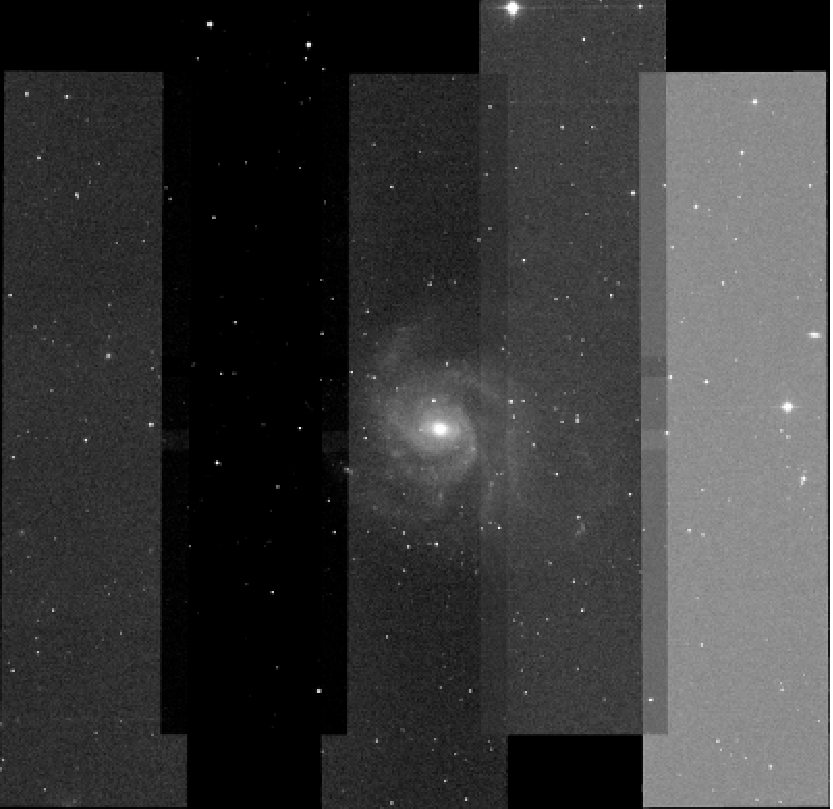
\includegraphics[scale=0.35]{imagens/mosaico1.pdf}
			\caption{Mosaico M101 não corrigido.}
			\label{fig:Mosaico}
		    \end{minipage}
		    \hspace{0.1cm} % To get a little bit of space between the figures
		    \begin{minipage}[b]{0.45\linewidth}
			\centering
			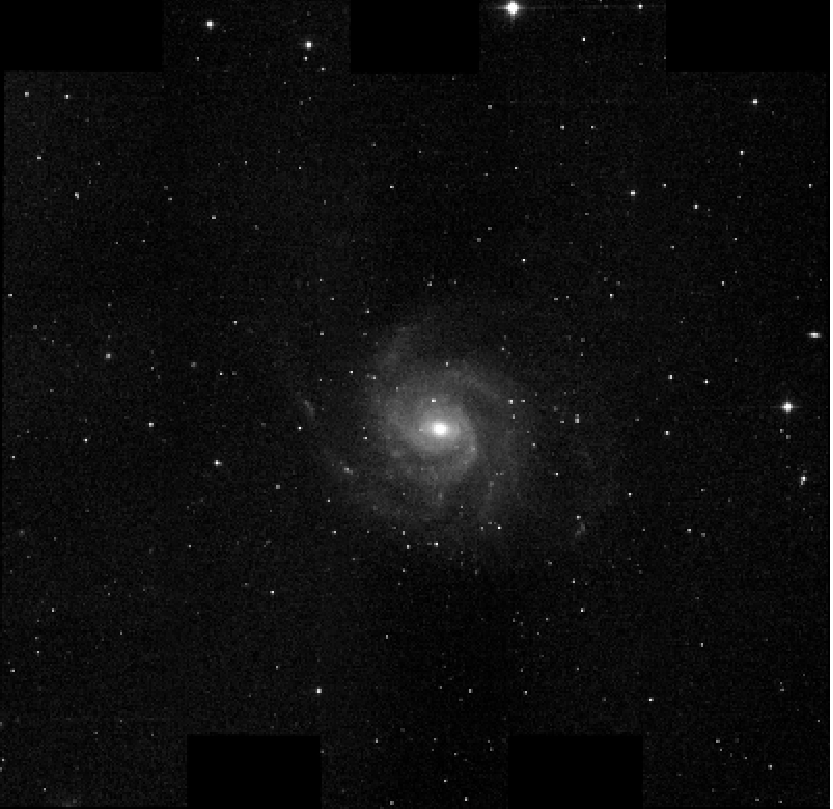
\includegraphics[scale=0.35]{imagens/mosaico2.pdf} 
			\caption{Mosaico M101 corrigido.}
			\label{fig:MosaicoCorrigido}
		    \end{minipage}
		\end{figure}
	    \end{center}
	\end{frame}
    
\section{Conclusões}
    \begin{frame}
	\begin{center}
	{\Huge Conclusões}
	\end{center}
    \end{frame}
    
    \subsection*{Conclusões}
    \begin{frame} \frametitle{Conclusões}
	\begin{itemize}
	    \item Abordagem do problema com WS-BPEL.
		\note[item] {A maioria dos trabalhos propõem novas linguagens.}
	    \item Foco na estrutura de CoC.
		\note[item] {Não foram encontrados trabalhos com como em CoC.}
	    \item Solução implementada de ponta a ponta se mostra viável.
		\begin{itemize}
		    \item Processo muitas vezes lento.
		    \item Complexidade para utilizar funcionalidades que não são comuns.
		    \item Dependente da máquina de execução utilizada.
		\end{itemize}
	\end{itemize}
    \end{frame}
    
    
    \begin{frame} \frametitle{Principais Contribuições}
	\begin{itemize}
	    \item As principais contribuições incluem:
	    \begin{itemize}
		\item Extensão à WS-BPEL para a especificação de \textit{workflows} em CoCs (WS-Policy);
		    \note[item] {Usando padrões consolidados, como o WS-Policy, permitindo a seleção de serviços baseada em requisitos não-funcionais;}
		\item Uma proposta de arquitetura para a execução de \textit{workflows} em um \textit{cluster} de \textit{clusters};
		\item Um estudo de caso aplicando essa arquitetura na rede SHARCNET;
		\item Uma implementação de escalonador global para a SHARCNET;
		\item Especificação e implementação de um \textit{workflow} científico real, utilizando o ambiente criado.
		    \note[item] {WF Real:= Mosaicos personalizados do céu}
	    \end{itemize}
	\end{itemize}
    \end{frame}
    
    \subsection{Trabalhos Futuros}
    \begin{frame} \frametitle{Trabalhos Futuros}
	\begin{itemize}
    	    \item Gerenciamento de dados e transferência de informações.
    	    \item Tolerância a falhas.
	    \item Ferramenta para auxiliar o monitoramento do estado de cada \textit{workflow} em execução.
	\end{itemize}
    \end{frame}
    
    \subsection{Publicações}
    \begin{frame} \frametitle{Publicações}
	\begin{itemize}
	    \item Posters e artigos resumidos:
		\begin{itemize}
		    \item ``\textit{A global scheduler for SHARCNET}''; \textit{SHARCNET Research Day 2009}; Waterloo, Ontário, Canadá.
		    \item ``\textit{Estendendo a linguagem WS-BPEL para a execução de workflows em um cluster de clusters}''; 4o Workshop de Teses de Doutorado UNICAMP, 2009; Campinas, Brasil.
		\end{itemize}
	\end{itemize}
    \end{frame}
           
    \begin{frame} \frametitle{Publicações}
	\begin{itemize}
	    \item Artigos completos:
		\begin{itemize}
		    \item ``\textit{An Infrastructure for Executing WS-BPEL Workflows in a Cluster of Clusters}''; \textit{IEEE symposium on Computers and Communications (ISCC 2010)}; Riccione, Itália.
		\end{itemize}
	\end{itemize}
    \end{frame}   
    
    \begin{frame} \frametitle{Palestras Aguardando Avaliação}
	\begin{itemize}
	    \item ``\textit{Orquestrando Serviços Web em Java com WS-BPEL}''; \textit{JavaOne: Oracle OpenWorld Latin America 2010}; São Paulo, Brasil.
	    \item ``\textit{Implementando Serviços Web Assíncronos em Java}''; \textit{JavaOne: Oracle OpenWorld Latin America 2010}; São Paulo, Brasil.
	    \item ``\textit{Orquestração de Serviços com WS-BPEL}''; \textit{Latinoware 2010}; Foz do Iguaçu, Brasil.
	\end{itemize}
    \end{frame}



 %Fim da apresentação
\section{}
\begin{frame}\frametitle{Agradecimentos}
\begin{itemize}
\item Prof. Maria Beatriz.
\item Prof. Miriam Capretz (UWO).
\item Membros da Banca.
\item Instituto de Computação.
\item FAPESP.
\end{itemize}
\end{frame}

\begin{frame}\frametitle{Obrigado!}
\begin{center}
{\Huge Dúvidas?}
\end{center}
\end{frame}

\startbackup
\appendix
\begin{frame}
\titlepage
Orientadora: Maria Beatriz Felgar de Toledo

Agência Financiadora: FAPESP
\end{frame}

\section{Backup}
    \begin{frame}
	\begin{center}
	{\Huge Backup}
	\end{center}
    \end{frame}

\begin{frame}\frametitle{Sumário}
\small\tableofcontents
\end{frame}

\subsection{SHARCNET}
\begin{frame}\frametitle{SHARCNET - HW}
  \begin{itemize}
    \item Three primary clusters that have already been listed in the top500 containing 267 nodes with 1068 processors, 768 nodes with 1536 processors and 768 nodes with 3072 processors
    \item Each of these clusters provides 70TB of high speed storage
    \item 17 secondary clusters, ranging from 32 to 64 nodes and totaling more than 8,000 processors and 200TB of storage
    \item Interconnection between the nodes in each cluster includes G2 Myrinet, Quadrics (Elan, Elan 4 and 3) and Gigabit Ethernet
    \item Communication between clusters is performed by a dedicated high-speed network and a 10 Gigabit Ethernet 
  \end{itemize}
\end{frame}

\begin{frame}\frametitle{SHARCNET - SW}
  \begin{itemize}
    \item Studies from many areas that traditionally require high performance computing: chemistry, physics, material science, and engineering;
and newer areas: business, economics and biology
    \item Operating systems are variants of Linux
    \item Job Scheduling is performed by the Load Sharing Facility (LSF)
    \item Parallel computing can be developed using MPI or OpenMPI
    \item Each cluster has a master node that acts as a local scheduler
  \end{itemize}
\end{frame}

\subsection{WS-PolicyAttachment}
\begin{frame}\frametitle{WS-PolicyAttachment}
WS-PolicyAttachment defines the attribute of a PolicyURI, which connects a WS-Policy to an XML element.
Accordingly, these attributes allow policies to be linked to WS-BPEL elements that represent service compositions or specific services in compositions. 
\end{frame}

\subsection{Correlação}
\begin{frame}\frametitle{Correlação}
    \begin{figure}[!htb]%Figura:Correlation
	\begin{center}
	    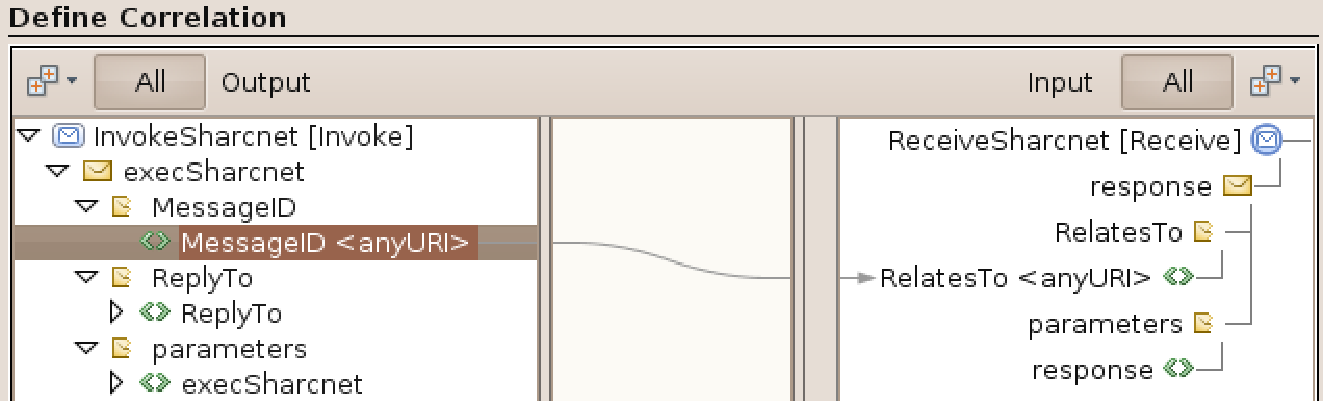
\includegraphics[scale=0.50]{imagens/Correlation.pdf} 
	    \caption{Estrutura de \texttt{Correlation} sendo criada.}
	    \label{fig:Correlation}
	\end{center}
    \end{figure}
\end{frame}


\subsection{Binding Dinâmico}
\begin{frame}[fragile]\frametitle{Binding Dinâmico}
O parâmetro \texttt{return}, da variável que recebe a saída do \texttt{Broker}, é atribuído ao parâmetro URL, das propriedades SOAP do serviço \texttt{ExecSharcnetIn}.
\begin{figure}[!htb]
    \centering
    \lstinputlisting[basicstyle=\tiny]{listings/bindingDinamico.xml}
    \caption{Configurando um \textit{binding} dinâmico.}
\end{figure}    
\end{frame}

\begin{frame}[plain]\frametitle{Binding Dinâmico}
    \begin{figure}[!htb]%Figura:Imagem BPEL M101
    \begin{center}
	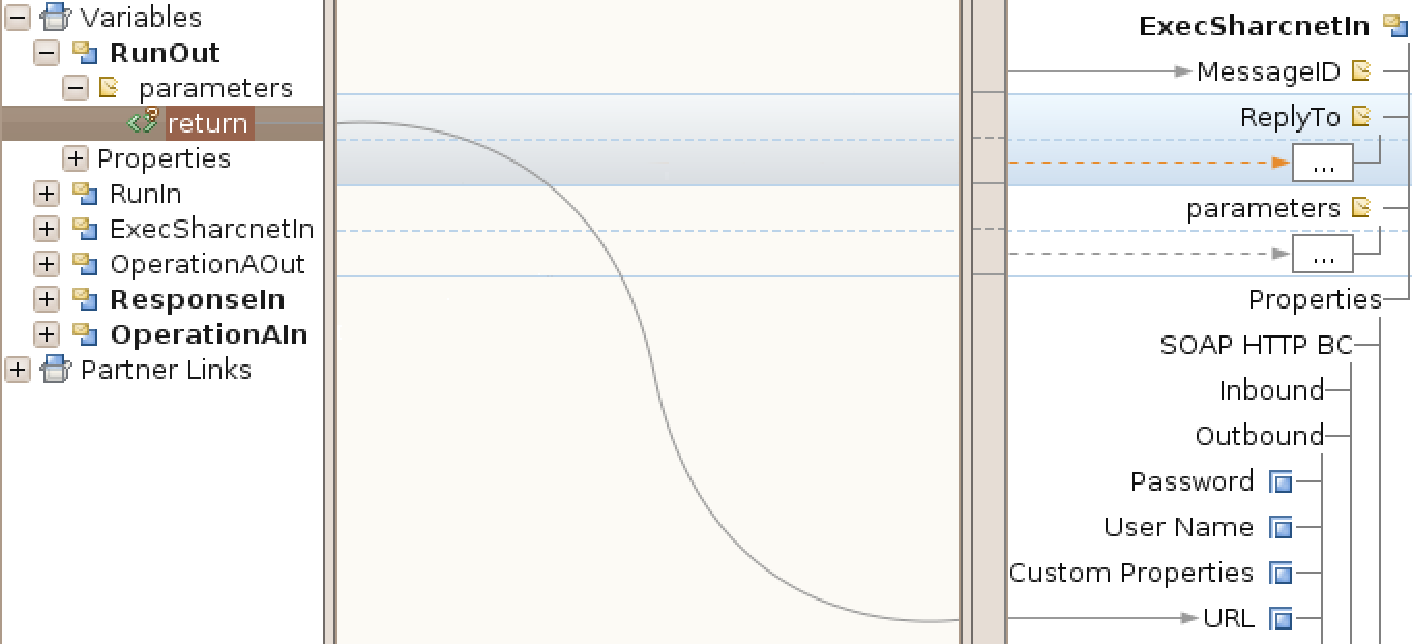
\includegraphics[scale=0.45]{imagens/BindingDinamico.pdf}
	\caption{Configurando um \textit{binding} dinâmico no Netbeans.}
    \end{center}
\end{figure}
\end{frame}

\subsection{Related Work}
\begin{frame}\frametitle{Related Work}
  \begin{itemize}
    \item Most authors agree that WS-BPEL can and should be adopted for grid service composition with some adjustments
    \item Many studies~\cite{GridServiceComposition08,Leymann06,GridEnabledWF08,Slomiski06,Tsalgatidou06}, consider the execution of workflows in OGSI (Open Grid Services Infrastructure) and WSRF grids
    \item Ezenwoye  et al.~\cite{GridServiceComposition08}, the authors focus on using BPEL to run WSRF services that implement the factory pattern
    \item Ma et al.~\cite{GridEnabledWF08} choose not to extend WS-BPEL, but to modify the ActiveBPEL engine instead
    \item Emmerich et al.~\cite{Emmerich05} use specifically GT3 and Cybok~\cite{Dieter06} uses Condor structures in their respective works
  \end{itemize}
\end{frame}

\begin{frame}\frametitle{Related Work - Cont.}
  \begin{itemize}
    \item Takpe et al.~\cite{Suter07}, as well as Qin and Bauer~\cite{Bauer07} demonstrate scheduling methods in a cluster of clusters
    \item Thus far, most of the proposals have been limited to formal proofs and/or simulations without implementation in a real environment
    \item Compatibility problem: This simple fact invalidates some proposals~\cite{Antonio09,Chau03}, which assume all requests are directed through the new "global scheduler"
    \item Hunold et al.~\cite{Rauber08} also propose a scheduling method for clusters using the technique of postponing: Starvation
  \end{itemize}
\end{frame}

\section{References}

	  \begin{tiny}	  
	  \bibliographystyle{plain}
	  \bibliography{../Referencial/Cluster-of-Clusters/coc,../Referencial/geral,../Referencial/BPEL-Grid/bpel-grid,../Referencial/WF-GRID/wf-grid,../Referencial/Sharcnet/sharcnet,../Referencial/WS/ws,../Referencial/SOA/soa}
	  \end{tiny}

%%%%%%%%%%%%%%%%%%%%%%%%%%FIM%%%%%%%%%%%%%%%%%%%%%%%


\end{document}